
\begin{abstract}
For the zero-stabilizer form of practical MaxRL with $N$ i.i.d.\ binary
rollouts, expected absolute coefficient mass is exactly
$2[1-(1-p)^N-p]=2(\passat{N}-\passat{1})$. This yields a rollout-aware
activity score, recovers $p(1-p)$ at $N=2$, and maps the drop-all-fail
convention to truncation order $N-1$. A fresh 20-seed Acrobot test supports
the deployed-$N$ score in one fixed task family. A separate 80-pair paid-probe
comparison does not support $u_{16}$ over source-faithful ProCuRL
environment selection ($\Delta=.0049$, $p=.0515$; SESOI $.02$), while probes
consume about 93.2\% of paid transitions and all probed arms trail ordinary
uniform by about $.31$ AUC. A fresh 24-block
exact-probability Digits counter-test does not support the registered
sampler-by-estimator interaction: RLOO reverses its predicted ordering and
both matched samplers underperform uniform. An externally recorded six-block
maze wave has higher MaxRL than GRPO coverage under each sampler, although its
locking object and checkpoint trajectories are absent here. A reported
three-seed Countdown aggregate moves mean@16 upward while the VERL bootstrap
best@16 proxy moves downward; that proxy is not standard unbiased
$\passat{16}$. Together, these positive and negative tests show that exact
coefficient activity can generate curriculum hypotheses but is not a
universal selection objective.
\end{abstract}

\paragraph{Status of this extended record.}
This file preserves the project's chronological research narrative and is not
the conference submission. The compact, claim-audited manuscript in
\texttt{body\_iclr.tex} is authoritative. Historical language below---including
``learnability functional,'' ``confirmation,'' and registration labels---must
be read through the current corrections: coefficient mass measures activity,
the Digits interaction is a registered negative, maze/Countdown timing objects
remain external, Countdown best@$k$ is a bootstrap proxy, and the separate
paid-probe ProCuRL-family comparison is a registered null dominated by probe
cost rather than evidence of general ProCuRL inferiority.

\paragraph{Countdown metric-provenance erratum.}
Historical sections and figures in this extended research record used the
logger's ``pass@$k$'' shorthand for
\texttt{pass@16\_accuracies/.../best@$k$/mean}. The VERL implementation
computes that field by 1,000 with-replacement resamples from the same 16
binary outcomes. Conditional on $c$ successes it estimates
$1-(1-c/16)^k$; it is neither the standard unbiased pass@$k$ estimator nor,
at $k=16$, simply the indicator of any observed success. The underlying
per-task outcomes are not vendored, so the standard metric cannot be
reconstructed. Until those outcomes are recovered, every historical
Countdown/Jugs pass@$k$ label below should be read as a bootstrap best@$k$
coverage proxy. The compact submission body uses the corrected terminology.

\section{Introduction}

Post-training language models and control policies with verifiable
rewards has a cost structure unlike supervised learning: the data is
free, but \emph{rollouts} are not. Every optimization step is preceded
by sampling $N$ completions per task, and generation can dominate
wall-clock --- in our committed telemetry, generation-dominated LLM
sessions average 83\% of step time.\footnote{Eight sessions, 282
steps; across all 1{,}188 logged steps including CPU-bottlenecked
maze-scale sessions the step-weighted mean is 31\% --- the 83\% figure
describes the LLM regime, not every workload.} On hard task pools,
most of that compute buys nothing: under uniform sampling we measure
that \textbf{65--75\% of rollout groups produce zero learning signal}
--- either every rollout fails (the group is dropped by
success-conditioned estimators) or every rollout succeeds (no
contrast, no gradient).

The field's response is a pair of data-level interventions. The first is
the \emph{difficulty curriculum}: reallocate the rollout budget toward
tasks where learning is possible right now --- UCB bandits over
difficulty buckets \citep{dump}, target-difficulty controllers
\citep{adarft}, category bandits \citep{sec}, learnability-based
rejection sampling \citep{lilo}, dead-prompt filtering \citep{dapo,greso}.
The second, newer, is \emph{failure recycling}: convert a failed rollout
into a verified success of the task it actually achieved --- hindsight
relabeling, recently brought into RLVR-style loops for robot policies
\citep{lfh}. Both interventions are, in current practice, designed and
evaluated as if they were \emph{objective-agnostic}: bolt-on modules
whose benefit is assumed to transfer across the advantage estimator they
sit on, and whose cost is assumed visible in the mean-accuracy metrics
they are tuned against.

This paper shows that neither assumption survives contact with the
estimator's own algebra. The organizing fact is the shape of one
function. \textbf{The estimator's derived utility $u_N(p)$ --- half
its expected coefficient mass --- vanishes exactly at pass rates $0$
and $1$ and peaks once in between, tracing three regimes of
difficulty: a dead zone, a learnable region, and a mastered tail. Curricula reallocate compute within the learnable
region; verified relabeling is a way to create a positive update for
an all-fail requested task; and relabels that land in the mastered
tail buy sharpening, not signal. The estimator shapes all three.}
Three questions unpack this:

\emph{Q1: What can a curriculum contribute, at most?} For
success-conditioned advantages, the expected coefficient mass a task
emits from a group of $N$ rollouts has a closed form:
$2(\passat{N}-\passat{1})$, a compute-indexed estimator-activity functional
whose two exact zeros anchor the difficulty regimes
(\S\ref{sec:theory}).
Mass is a surrogate for learning signal (Remark~\ref{rem:scope}), but
it is the part a sampler can act on before spending a rollout, and it
makes the allocation \emph{derivable} rather than heuristic: the
activity region's location, peak, and $N$-scaling come from the
budget you already
chose, and several variance-based curricula use the same $N{=}2$ shape. It
also bounds the channel. Allocation can only redistribute signal that
exists: a perfect-information allocator ties the full
posterior-plus-recycling stack in end performance (\S 6.1) --- so
recycling compensates for allocation error rather than beating perfect
allocation --- and at LLM scale a prompt-level teacher starves before
it pays (\S\ref{sec:experiments}).

\emph{Q2: When is either intervention safe?} The same algebra says the
answer depends on the estimator. MaxRL concentrates $(N{-}1)\times$
more mass than RLOO (the unnormalized leave-one-out baseline
estimator) on hard tasks as $p \to 0$ and releases mastered tasks;
GRPO's variance-normalized weights keep spending on both tails. The
predicted coverage ordering is robust where gradients are exact; at
neural scale the first factorial \emph{retired its strong form} --- an earlier
cohort's zero-exception divergence had conflated recycling's contribution with
the estimator effect. According to the external execution record, the
time-integrated outcome was specified before a second factorial on fresh seed
blocks and met its stored directional rule in 6/6 paired blocks under each
sampler. The locking object is absent from this checkout, so the timing is
reported rather than independently auditable. The pair-level easy-band bar was met, but its
block-level interval includes zero, so the localization remains
suggestive (\S 6.3b tells that story once, in full). Countdown provides
a narrower warning: in three-seed aggregates, exact-verifier recycling raises
mean accuracy while the logged VERL bootstrap best@16 coverage proxy falls.
The standard pass@$k$ direction is unknown because task outcomes are missing,
and concentration on reachable destinations remains a mechanism hypothesis.
A higher-dose live-group arm improves both logged metrics but does not identify
the relabel direction or define a causal bound (\S 6.8).

\emph{Q3: Does the algebra suggest a fix?} It motivates one. A
relabel to a destination the model reliably reaches sits in the
mastered tail, where mass vanishes, so we gate relabel admission by a
saturation statistic on the destination --- a decayed frequency over
the recycler's own recent relabel stream. The mastered-tail zero
motivates \emph{that such a threshold should exist}; the statistic
itself is a tuned heuristic, not a destination pass-rate estimate
(\S 6.9 states exactly what it is and is not). An under-gated
three-seed setting returned frontier-tier coverage to baseline while
keeping most of the mean gain, but a corrected-code strong setting
failed; we therefore report the gate as a secondary heuristic, not a
validated contribution. Each domain also supplies a relabel map and a
destination key, and Jugs showed that key choice is load-bearing
(\S\ref{sec:limits}).

Our contributions:
\begin{enumerate}
\item \textbf{A closed-form estimator-activity functional}
  (\S\ref{sec:theory}): the expected coefficient mass of a prompt
  under success-conditioned RL is exactly $2(\passat{N}-\passat{1})$,
  compute-indexed, with peak location and $N$-scaling derived rather
  than tuned, and exact zeros at $p\in\{0,1\}$ anchoring the dead
  zone, the learnable region, and the mastered tail; several variance-based
  curricula use the same $N{=}2$ shape. (The functional is
  closed-form; the sampler built on it still estimates $p$ and keeps
  standard knobs.) A fresh fixed-pool score test supports the deployed-$N$
  shape, while a separate 80-pair paid-probe family does not support
  $u_{16}$ over ProCuRL selection and exposes probe-cost domination at its
  frozen cadence.
\item \textbf{A controlled estimator-conditioned coverage result}
  (\S\ref{sec:experiments}): the first factorial retired the cohort's
  zero-exception divergence. According to the external execution record, the
  surviving time-integrated ordering was specified before a second factorial
  on fresh seed blocks and met its stored 6/6 directional rule under both
  samplers ($p{=}.031$ each); the locking object is absent here.
  Sampler-averaging within independent blocks gives a positive
  interval in wave 2 and 12/12 positive blocks descriptively across
  waves; the easy-band localization remains suggestive.
\item \textbf{An applied accuracy--proxy tradeoff}
  (\S 6.8--6.9): the reported three-seed recycling aggregate has higher
  mean@16 and lower VERL bootstrap best@16. Missing paired records and task
  outcomes preclude per-seed inference or a standard pass@16 claim. A
  higher-dose live-group alternative improves both logged metrics without
  isolating relabel direction, and a corrected-code gate falsification limits
  the proposed mitigation.
\end{enumerate}
Along the way we state a refinement to the MaxRL paper --- the practical
drop-$K{=}0$ estimator is unbiased for the $T{=}N{-}1$ objective, not
$T{=}N$ (Lemma~\ref{lem:trunc}) --- and catalog the available timing evidence,
negatives, and retractions in place (\S\ref{sec:limits}) and in the repository;
App.~\ref{app:claims} tabulates every load-bearing claim with its
evidence and registration status.

\begin{figure}[t]
\centering
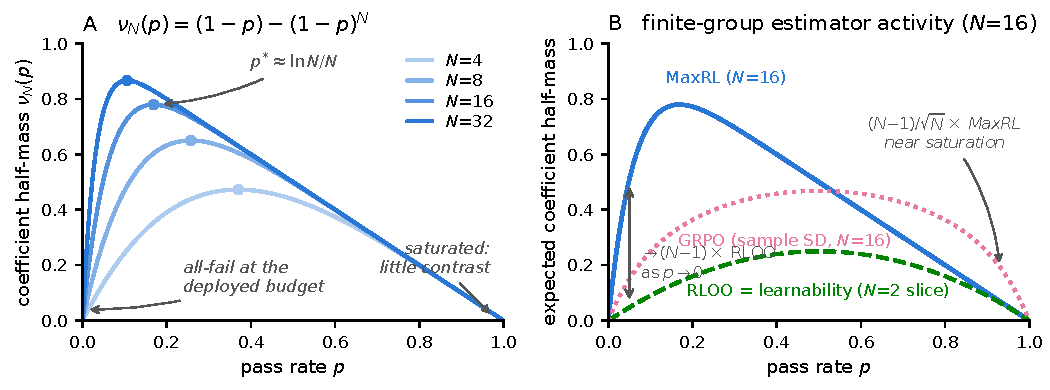
\includegraphics[width=0.92\linewidth]{figures/fig1_utility}
\caption{\textbf{The estimator is the curriculum.} \emph{Left:} the derived
utility $u_N(p) = (1-(1-p)^N)-p$ --- half the estimator's expected
coefficient mass $A_N = 2u_N$ (Prop.~\ref{prop:mass}) --- for growing
rollout budgets $N$. The peak $p^*\approx \ln N/N$ walks toward harder
prompts as compute grows; the utility vanishes exactly at $p\in\{0,1\}$.
\emph{Right:} all three curves are exact expected half-mass at $N{=}16$
for the estimators \emph{as deployed} (GRPO with sample-SD
normalization:
$\sqrt{\tfrac{N-1}{N}}\,\frac{1}{N}\mathbb{E}\sqrt{K(N{-}K)}$,
$K\sim\mathrm{Bin}(N,p)$; MC-verified against the code). MaxRL
concentrates $\to(N{-}1)\times$ more mass than RLOO on frontier prompts
(Prop.~\ref{prop:ratio}); in the mastered tail MaxRL and RLOO decay
together at first order (both $\to q = 1-p$; MC artifact
\texttt{verify\_guidance\_math.json}) while GRPO's variance
normalization keeps ${\sim}(N{-}1)/\sqrt{N}\times$ their relative mass
there --- the maintenance-of-easy-tasks its curriculum arms lose in
\S\ref{sec:experiments}. RLOO's profile is
exactly the published ``learnability'' objective --- the $N{=}2$
slice.}
\label{fig:utility}
\end{figure}

\section{Background: MaxRL in three lines}
For binary rewards, maximum likelihood maximizes
$\mathbb{E}[\log p_\theta(\text{success}\mid x)]$. MaxRL expands $\log p$
as a Maclaurin series in $(1-p)$ and truncates at order $T$, giving a
compute-indexed family $J^{(T)}$ interpolating REINFORCE ($T{=}1$) to exact
ML ($T\to\infty$); the practical estimator sets per-rollout advantages
$w_i = r_i/K - 1/N$ with all-fail groups dropped
(Lemma~\ref{lem:trunc} gives its exact truncation order). Its weight
function grows as $p\to 0$: the objective
is an \emph{implicit, gradient-level} curriculum. Our work is the
data-level complement: the same algebra, read as a sampling rule plus a
recycling rule.

\section{The estimator is the curriculum}\label{sec:theory}

\begin{lemma}[Truncation order of the practical estimator]
\label{lem:trunc}
Let $J_T(p) = -\sum_{t=1}^{T}(1-p)^t/t$ denote the $T$-truncated ML
objective, so $\nabla J_T = \big(\sum_{j=0}^{T-1}(1-p)^j\big)\nabla p$;
$T{\to}\infty$ recovers exact ML and $T{=}1$ REINFORCE. Under $N$
i.i.d.\ binary rewards with pass rate $p$, the drop-$K{=}0$ variant of
the practical MaxRL estimator has expectation
$\big(\tfrac{1-(1-p)^N}{p} - (1-p)^{N-1}\big)\nabla p
= \big(\sum_{j=0}^{N-2}(1-p)^j\big)\nabla p$: it is exactly unbiased
for $J_{N-1}$, not $J_N$, for $N \ge 2$. Zeroing the control variate
only on all-fail groups makes it outcome-dependent, contributing the
$-(1-p)^{N-1}\nabla p$ correction, and
$\sum_{k=1}^{N}(1-p)^{k-1} - (1-p)^{N-1} = \sum_{k=1}^{N-1}(1-p)^{k-1}$.
\end{lemma}
\begin{interp}
Three estimators must be kept distinct: the \emph{raw}
success-conditioned average ($\frac{1}{K}\sum r_i S_i$, no control
variate --- the object of \citet{maxrl}'s Theorem 2, exactly unbiased
for $J_N$), the \emph{full control-variate} form (subtracting the
unconditional mean score on every group, including all-fail ones), and
the \emph{practical drop-$K{=}0$} form above, which is what ships.
The lemma is a refinement to \citet{maxrl}, immaterial for their
conclusions but load-bearing for our mass accounting at small $N$ ---
all identities below are for the estimator as actually shipped.
Magnitude at the
deployed budgets: the relative gradient shortfall of $T{=}N{-}1$ vs.\
$T{=}N$ is $(1-p)^{N-1}/\sum_{k=1}^{N}(1-p)^{k-1}$ --- at $N{=}16$ it
is $5.8\%$ at $p{=}.01$, $1.1\%$ at the band peak $p^*{\approx}.17$,
and ${<}10^{-4}$ at $p{=}.5$; at $N{=}8$ it reaches $12\%$ on the deep
frontier. Bookkeeping at moderate $p$, material exactly where the
frontier teacher concentrates sampling.
\end{interp}

\begin{proposition}[Expected coefficient mass]\label{prop:mass}
For a prompt with pass rate $p$ and $N$ i.i.d.\ rollouts under the
practical MaxRL weights, define the utility
$u_N(p) := \passat{N}(p) - \passat{1}(p) = (1-(1-p)^N) - p$. Then the
expected absolute coefficient mass is
\begin{equation}\boxed{\;
A_N(p) \;:=\; \mathbb{E}\Big[\textstyle\sum_i |w_i|\Big]
   \;=\; 2\big(\passat{N}(p) - \passat{1}(p)\big)
   \;=\; 2\,u_N(p).\;}
\label{eq:mass}
\end{equation}
Proof (three lines): on $\{K\ge 1\}$,
$\sum_i|w_i| = K(\tfrac1K - \tfrac1N) + \tfrac{N-K}{N} = 2(1-\tfrac KN)$,
and $\mathbb{E}[2(1-\tfrac KN)\mathbf 1\{K\ge1\}]
= 2(\Pr[K\ge1] - p) = 2(\passat{N}-\passat{1})$. The sampling utility
used everywhere below (figures, Algorithm~\ref{alg:frontiermax}, code)
is $u_N$; the factor two matters only when quoting exact mass, and we
carry it explicitly as $A_N = 2u_N$. Two exact companions tie mass to
the gradient. \emph{Factorization}: writing $\mu_{\pm}(x) =
\mathbb{E}[S \mid r{=}1/0, x]$ for the success/failure-conditioned
score means, exchangeability gives, for every group size,
\begin{equation}
\mathbb{E}[\hat g \mid x] \;=\; u_N(p)\,\big(\mu_+(x) - \mu_-(x)\big),
\label{eq:factorization}
\end{equation}
so $u_N$ is exactly the estimator-controlled scalar multiplying the
prompt's success--failure score contrast --- the part of the expected
update a sampler can know before rolling out; the contrast (and where
it transfers) is the part it cannot. \emph{Weight view}: since
$\mu_+ - \mu_- = \nabla p/(p(1-p))$,
Eq.~\eqref{eq:factorization} is equivalent to
$u_N(p) = p(1-p)\,w_{N-1}(p)$ with $w_T(p) = (1-(1-p)^T)/p$ the
truncated weight function of Lemma~\ref{lem:trunc} --- mass and the
practical estimator's weight view are linked, not identical objects.
(Both identities MC-verified; artifact
\texttt{verify\_guidance\_math.json}.)
\end{proposition}
\begin{interp}
The estimator's expected coefficient mass on a prompt is twice the
probability that the prompt is solvable within $N$ attempts but not
within one. Coefficient mass is a \emph{surrogate} for learning signal
(Remark~\ref{rem:scope}), but its two zeros are exact, and they anchor
three regimes of difficulty. A \emph{dead zone} at $p = 0$: nothing to
condition on; sampling alone cannot produce a success
there.\footnote{At small $p > 0$ a task is \emph{operationally} dead
at budget $(B,N)$ when its live-group probability
$1 - (1 - \ell_N(p))^{B}$, with $\ell_N(p) = 1 - p^N - (1-p)^N$ and
$B$ its share of groups, is too small to sustain training. On the
frontier-heavy pool of \S 6.2 ($p \le 10^{-5}$, ${\sim}133$ groups per
task) that probability is ${\le}2\%$ per task, and the one live group
observed across all uniform seeds did not ignite --- dead in the
budgeted sense, not by fiat.} A \emph{learnable region} with a unique
interior peak at $p^* = 1 - N^{-1/(N-1)} \approx \ln N/N$ (unique
because $u_N'' < 0$). A \emph{mastered tail} at $p = 1$: no contrast
left. The regimes are continuous --- the only exact zeros are
$p \in \{0,1\}$ --- so where we quote a ``band'' we mean the threshold
set $\{p : u_N(p) \ge \eta\, u_N(p^*)\}$ ($\eta{=}0.5$ unless stated),
whose location and $N$-scaling follow from the one parameter you
already chose. Everything in this paper is one of three moves against
this structure: allocate within the learnable region
(\S\ref{sec:method}), create signal at its bottom
(\S\ref{sec:recycling}), and refuse updates that land in the mastered
tail (the gate).
\end{interp}

\begin{proposition}[Frontier amplification]\label{prop:ratio}
As $p \to 0$, the ratio of MaxRL's expected mass to RLOO's
($A_N^{\mathrm{RLOO}} = 2p(1-p)$ exactly, under the $1/N$-normalized
leave-one-out weights) tends to $N-1$.
\end{proposition}
\begin{interp}
The comparison to GRPO is two-sided and exact in the $\varepsilon\to0$
form of the deployed implementation, which normalizes by the \textbf{sample}
standard deviation ($s_K = \sqrt{K(N{-}K)/(N(N{-}1))}$, PyTorch's default),
not the population SD. The released code uses $s_K+10^{-6}$; this makes a
numerically negligible but formally distinct curve:
$A_N^{\mathrm{GRPO}}
= 2\sqrt{\tfrac{N-1}{N}}\,\frac{1}{N}\mathbb{E}\sqrt{K(N{-}K)}$
with $K\sim\mathrm{Bin}(N,p)$ (MC-verified against
\texttt{estimators.py}). Taking tails, MaxRL/GRPO $\to \sqrt{N}$ as
$p\to 0$ while GRPO/MaxRL $\to (N{-}1)/\sqrt{N}$ as $p\to 1$
(at $N{=}16$: $4.0\times$ and $3.75\times$; the symmetric
$\sqrt{N{-}1}$ holds only under population-SD normalization). MaxRL
over-serves the frontier and releases mastered prompts; GRPO silently
keeps ${\sim}(N{-}1)/\sqrt{N}\times$ more of its mass on mastered
prompts --- maintenance a curriculum then removes. One caveat governs
every cross-estimator magnitude in this paper, and we measured its
bite: each estimator's coefficients carry a conventional global scale
(absorbable into the learning rate), so absolute ratios like these
are facts about the implementations as shipped under a common
learning rate, not invariant properties of the objectives --- and on
a learnable-everywhere pool an lr sweep shows a $2$--$4\times$ raise
lets GRPO match MaxRL's raw coverage \emph{delta} (though not its
coverage--reliability premium; \S 6.3b). What survives any
recalibration is the \emph{shape}: where each estimator's mass
concentrates as a function of $p$, and its exact zeros --- which is
why the empirical claims are about tails, signs, and
premium-vs-reliability trades, not magnitudes. Concentrating sampling on the frontier only helps if the
estimator extracts signal there, and \S\ref{sec:experiments} shows
the mastered-tail difference becoming an active failure under a
curriculum.
\end{interp}

The static known-$p$ allocation problem this utility induces has a
clean water-filling solution, but the deployed teacher does not use
it (it keeps fixed group sizes and samples $\propto u^\gamma$ with a
floor, trading myopic optimality for group-parallel batching and
exploration); we state the allocator and its boundary conditions in
App.~\ref{app:alloc} and measure what the gap costs in \S 6.1, where
a no-floor, $\gamma$-matched true-pass-rate oracle ties the Thompson
teacher in end performance.

\begin{remark}[Scope of the surrogate]\label{rem:scope}
Coefficient mass counts weighted rollouts, not score-vector geometry. We
use it as the sampling utility because (i) it is knowable \emph{before}
spending rollouts, (ii) its zeros are exact --- at $p\in\{0,1\}$ the
estimator emits no gradient of any norm --- and (iii) on the
exact-gradient testbed it \emph{ties} the true first-order expected
improvement as a task ranking (Spearman within $.005$ at every
snapshot, and exactly $1.0$ against the full exact transfer matrix ---
one expected group per task, exact $\Delta p$ on every other task ---
at three training snapshots; artifacts \texttt{results\_bridge.json},
\texttt{results\_transfer\_matrix.json}). That tie is a property of
\emph{shared-prefix} task structure, where activity and transfer
align; on pools without it, activity ranks what a task can emit, not
where it helps (\S 6.5--6.6 measure that gap). What it does not
claim to be is \emph{the} optimal sequential utility, and no
state-local functional is: on independent tasks the true
final-performance optimum is a planning solution (trajectory-knapsack
with a budget-dependent funding cutoff), and which surrogate best
approximates it depends on the training objective --- a
variance-tilted $(1{-}p)^\alpha u_N$ wins anytime performance while
model-predictive replanning wins the final checkpoint, each losing the
other's metric (8--10/10 paired seeds each way; App.~\ref{app:rungs}).
``Best curriculum utility'' is ill-posed until that objective is
fixed; we report both currencies throughout. The claim that carries the section
is the pair of exact zeros at $p\in\{0,1\}$, which every candidate
utility shares --- though the zeros alone do not suffice: a
uniform-over-band control (sample the in-band indicator, discard the
shape) forfeits most of the allocation gain on chains ($0.681$ vs.\
$0.743$ AUC, 0/10 seeds; artifact \texttt{results\_bridge.json}).
$u_N$'s standing is therefore: the shape matters, the best shape is
objective- and testbed-dependent, and $u_N$ is the one shape that
ties the exact first-order objective as a predictor, requires no
tuning, and transfers to the maze within noise.
\end{remark}

\begin{remark}[The curriculum changes the training distribution]
\label{rem:objective}
Sampling prompts from an adaptive $q_t$ instead of the data
distribution $\rho$ optimizes a reweighted objective
$\mathbb{E}_{x\sim q_t}[J(x)]$: each group's gradient is an unbiased
MaxRL gradient \emph{for its own prompt}, but the mixture is tilted
toward the frontier, without importance correction back to $\rho$.
This is the standard bargain every curriculum strikes (uniform
sampling makes the same choice for $q_t{=}\rho$), and we treat it as
an empirical question, not a free lunch: all evaluations in
\S\ref{sec:experiments} are on fixed held-out pools under $\rho$, so
any mismatch cost is charged to the method. The safety results are
precisely about when this tilt helps or hurts the $\rho$-measured
outcome.
\end{remark}

\noindent One identity, three literatures: learnability curricula
\citep{sfl,lilo} are the $N{=}2$ slice of $u_N$; DAPO-style dynamic
sampling and GRESO are its avoidance shadow (cull where $u\approx 0$);
HER-style relabeling \citep{her} is its creation complement
(manufacture $K>0$ where $u=0$ identically; \S\ref{sec:recycling}).
DisCO \citep{disco} and SC-SDPO \citep{scsdpo} derive analogous
per-question weights for the GRPO family to diagnose difficulty bias;
our identity generalizes that line to success-conditioned estimators
and --- the step neither takes --- uses it to predict how
\emph{external} curricula and recyclers interact with each estimator,
in coverage terms.

\paragraph{The three regimes, as a map of the paper
(Fig.~\ref{fig:channels}).} The \textbf{teacher}
(\S\ref{sec:method}) allocates compute within the learnable region ---
and saturates: a true-pass-rate oracle allocator ties the cheap
posterior in end performance (\S 6.1), so better pass-rate information
is not where remaining gains live. \textbf{Recycling}
(\S\ref{sec:recycling}) creates signal where sampling the requested
task yields none --- in our control battery, the one intervention
that still adds on top of the oracle. The \textbf{estimator}
underneath shapes whether either is safe, and its mastered tail is
where both failure modes live (\S\ref{sec:experiments}). One line:
\emph{the teacher allocates, hindsight creates, the estimator decides
whether either is safe} (Fig.~\ref{fig:algorithm}).

\begin{figure}[tb]
\centering
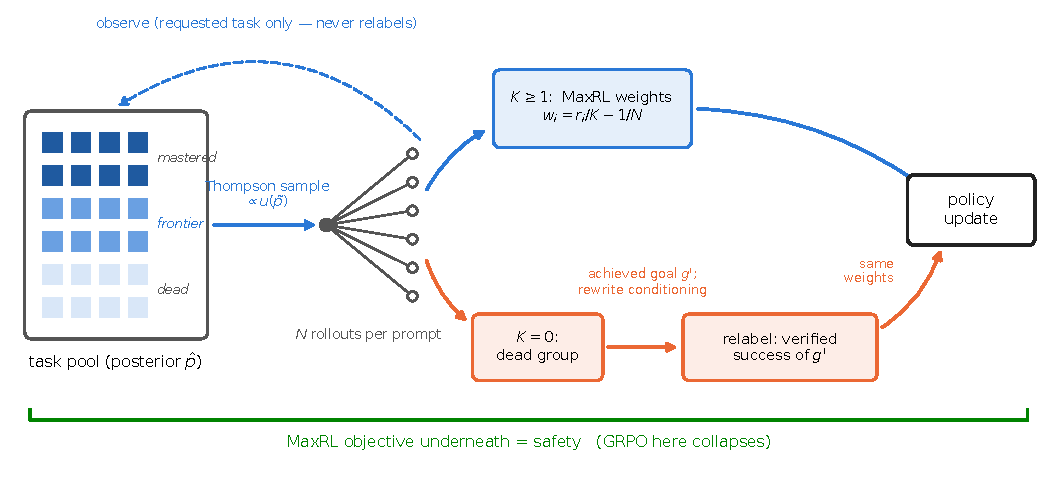
\includegraphics[width=0.85\linewidth]{figures/fig4_algorithm}
\caption{\textbf{One FrontierMax step.} A Thompson-sampled posterior
allocates rollouts by the derived utility; live groups train with
unmodified MaxRL weights; dead groups are relabeled to the sub-goal they
actually achieved (conditioning rewritten) and train as verified successes.
The posterior observes requested-task outcomes only.}
\label{fig:algorithm}
\end{figure}

\section{FrontierMax: the schedule}\label{sec:method}
FrontierMax is a standard group-rollout RLVR loop with three modified
lines (Alg.~\ref{alg:frontiermax}). A decayed Beta posterior tracks
each prompt's pass rate from observed group outcomes only --- never
from relabeled successes, which inflate it ($\hat p$ 0.81 vs.\ eval
0.47). Thompson sampling draws $\tilde p$ and samples prompts
$\propto u(\tilde p)^\gamma$ with a uniform floor. The knobs (decay
0.7, floor 0.1, $\gamma \in \{1, 4\}$) carry validated defaults
(Table~\ref{tab:knobs}); what is \emph{derived} rather than tuned is
the difficulty band itself --- location, width, and $N$-scaling ---
which is exactly where competing curricula spend their
hyperparameters.

\begin{algorithm}[tb]
\caption{FrontierMax: one step. Three lines differ from a standard
group-rollout loop (marked $\triangleright$).}
\label{alg:frontiermax}
\begin{algorithmic}[1]
\STATE $\triangleright$ \textbf{sample} prompts $x_1..x_B \propto
  u_N(\tilde p_x)^\gamma$ mixed with a uniform floor, $\tilde p_x \sim
  \mathrm{Beta}(\alpha_x, \beta_x)$ \hfill(else: uniform)
\STATE roll out $N$ completions per prompt; verify; $K_x \gets$
  successes
\STATE update posterior $(\alpha_x, \beta_x)$ from $(K_x, N)$
  \emph{for the requested task only}
\STATE live groups ($1 \le K_x$): MaxRL advantages
  $w_i = r_i/K - 1/N$, unchanged
\STATE $\triangleright$ \textbf{dead groups} ($K_x{=}0$): relabel each
  parseable failure to \emph{its own} achieved sub-goal $g'$
  (verified; conditioning rewritten); unparseable rollouts stay
  failures, so the group retains contrast ($K < N$)
\STATE $\triangleright$ \quad admit the relabel only if
  $\hat f_{g'} \le$ \texttt{gate\_max\_p}, where $\hat f_{g'}$ is a
  decayed frequency of $g'$ in the recycler's recent relabel stream
  (recorded whether or not admitted) \hfill(the gate: refuse
  recently seen destinations; never-seen destinations start at the
  Beta(1,1) prior $\hat f = .5$, admitted at the default threshold)
\STATE one policy-gradient step on live $+$ admitted relabeled groups
\end{algorithmic}
\end{algorithm}

\section{Failure recycling}\label{sec:recycling}

\begin{remark}[Hindsight update, characterized]\label{prop:hindsight}
Relabeling a dead group to the sub-goal $g'$ its trajectories actually
achieved, rewriting the goal conditioning, and applying the same
success-conditioned weights yields a \emph{verified weighted-likelihood
update for the achieved task}: every relabeled example is a true
success of $g'$ under the environment's verifier. It is generally an
\emph{adaptively selected, off-policy auxiliary update}, not an
unbiased gradient of $g'$'s on-policy objective: $g'$ is selected from
the same group being scored, conditioning on the requested task's
failure correlates the rollouts, the conditioning rewrite changes the
law under which the log-probability is evaluated, no importance ratio
corrects for it, and the finite-$N$ weights target $J_{N-1}$
(Lemma~\ref{lem:trunc}) rather than exact ML. It equals the
fresh-rollout $J_{N-1}$ gradient for $g'$ only under a
distribution-matching condition --- the selected, rewritten group must
have the same joint law as an i.i.d.\ fresh rollout group for $g'$.
This specializes known relabeling-bias structure --- the
induced-distribution view of \citet{eysenbach} and the
conditional-law gap in \citet{gcsl} --- to success-conditioned RLVR
weights; we state it as a remark, not a result, and note that the
sharpening phenomenon of \S 6.8 runs through the \emph{marginal}
shift those works also identify, not this conditional matching.
One further gap separates this remark from the deployed LLM loop:
the remark is written for a group with \emph{one} destination $g'$,
but Algorithm~1 relabels each parseable failure to \emph{its own}
achieved goal, so one group can mix rewritten tasks --- and once
destinations differ within a group, the shared success count $K$
couples unrelated tasks and the update is not a $J_{N-1}$ gradient
for \emph{any} single achieved task. We therefore read the deployed
per-row variant as a \emph{verified weighted-SFT update}, treat its
results as evidence about that objective, and measure the coupling's
cost where all variants are exactly implementable: per-row relabels
as their own $K{=}1$ groups lead (AUC $.952$),
one-destination-per-group is next ($.881$), and the shared-$K$
coupled form forfeits most of recycling's value ($.749$ vs.\
no-recycling $.705$; both orderings 10/10 paired seeds; artifact
\texttt{results\_row\_vs\_group.json}). Full object-level
characterization, the CPU-reference contrast, and the LLM-side
ablation flag: App.~\ref{app:mixed}.
\end{remark}
\begin{interp}
``Exactness'' is a property to \emph{measure per environment}, not a
blanket guarantee. We measured the two gaps the remark names where
they are measurable (exact chains, 5 seeds; artifact
\texttt{results\_proposal\_shift.json}): the applied relabel update's
cosine against the exact fresh-destination gradient is $0.93$; the
selection bias on the destination's success rate is small here
($+.003$); and cross-fitting the destination choice removes the
adaptive reuse at a real cost (alignment $\to 0.82$, AUC
$.883\to.829$). The off-policy caveat is real; its sign is
environment-specific.
\end{interp}

Two contracts keep practice on the proof's side: \textbf{(1)
exactness} --- a relabeled success must be a true success of the
relabeled task under the environment's own verifier (never an LLM
judge); \textbf{(2) conditioning} --- goal-embedding trajectories must
have their conditioning rewritten to the achieved goal. Skipping (2)
turns the exact gradient into noise: on our gridworld, hindsight
without the rewrite scores below teacher-only ($0.600 < 0.658$); with
it, it leads ($0.703$). Among the interventions studied here,
recycling is the one that \emph{creates} signal for an all-fail
requested task (adding the achieved sub-goals to the pool by hand
would too --- what recycling buys is discovering them, \S 6.2), and we
decompose its headline gain rather than
let it inflate: of the $+0.22$ AUC on fixed task pools, a placebo
replaying \emph{live} gradients on dead-group slots captures 83\% ---
most of the benefit is extra gradient dose on otherwise-wasted slots
--- while the relabel \emph{direction} carries $+0.037$ beyond the
strongest placebo, is the tightest arm in the battery, and is
exactness-dependent (random-target relabels lose to dose-matched
replay 5/5). Both numbers ship together --- and the same replay control,
transplanted to LLM scale as a pre-registered dose arm, makes the
sign starker: there it exceeds recycling on \emph{both} meters,
3/3 seeds (\S 6.8). The
value is regime-dependent in a way we can state precisely: $+0.22$
AUC on fixed task pools, $+0.01$ on one-shot task streams --- the
gain is proportional to how much a relabeled skill can compound, and
task-set fixedness is the single most important regime variable we
found.

\begin{figure}[tb]
\centering
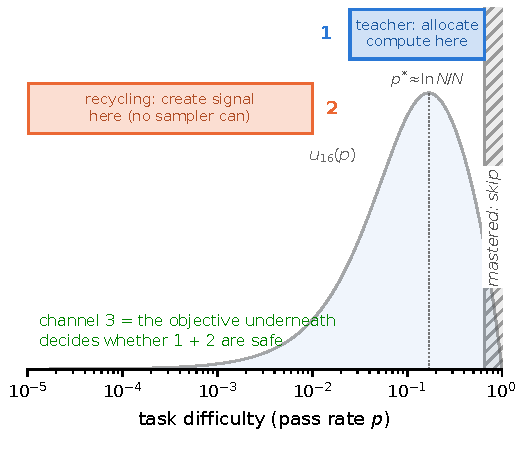
\includegraphics[width=0.5\linewidth]{figures/fig5_channels}
\caption{\textbf{The three regimes as a map of the method.} The teacher
allocates compute within the learnable region; recycling creates
signal where sampling the requested task yields none; the gate refuses
relabels that land in the mastered tail; the estimator underneath
decides whether any of it is safe.}
\label{fig:channels}
\end{figure}

\section{Experiments: an escalating ladder}\label{sec:experiments}

Each rung asks one question of the three-regime structure, at
increasing scale and decreasing experimental control;
Table~\ref{tab:ladder} is the map. Statistical contract, stated once
and used throughout: the independent unit for any training-method
claim is an independently trained seed block; runs sharing a seed,
warmstart, or checkpoint are paired or correlated observations, never
additional replicates; levels, $k$ values, metrics, and checkpoints
from one trained model are repeated measurements of it;
repeated-evaluation spread measures evaluation noise, not
training-seed uncertainty, and every $\pm$ names its source at point
of use ($\pm$ with no qualifier is standard deviation across training
seeds). Maze ``coverage'' is standard $\passat{k}$ with exactly $k$
samples per prompt. The VERL-backed Countdown, GSM8K, and Jugs logs instead
store a with-replacement bootstrap best@$k$ proxy under their historical
pass@$k$ key; the metric erratum above governs those sections. Mean@$k$ is
the mean success fraction of the same $k$ samples; AUC is the mean of the eval
curve over training at matched wall-clock or episode budget, and
final is the last checkpoint. Where run pools are heterogeneous we
say so and report signs descriptively rather than attaching $p$-values
(\S 6.3--6.4). External execution records label several predictions as
specified before their deciding runs, but the corresponding locking objects
are not all vendored; the compact paper discloses that timing limitation.
Negative results remain in the repository's audit trail.

\begin{table}[t]
\centering\scriptsize
\setlength{\tabcolsep}{3pt}
\caption{The ladder at a glance: every rung asks one question of the
three-regime structure; scale rises, control falls.}
\label{tab:ladder}
\begin{tabular}{@{}lllll@{}}
\toprule
rung & question & setting & seeds & outcome \\
\midrule
6.1 & does allocation saturate? & skill chain (exact grads) & 5 &
yes: oracle ties posterior \\
6.2 & anything to sample toward? & frontier-heavy pool & 5 &
no: only creation scores \\
6.3a & does the curriculum pay? & maze cohort, 1.26M & 3 &
throughput + recycling signal \\
6.3b & estimator effect, real grads? & maze factorial & 6 blocks &
endpoint failed; AUC 6/6/sampler \\
6.4 & where/when does coverage go? & maze, level-resolved & 22 runs &
easy band, immediately \\
6.5$^{*}$ & when does allocation not pay? & IsaacLab Anymal-C & 1 &
learnable-everywhere: null \\
6.6$^{*}$ & beyond task spread? & MountainCar/CartPole & 3 &
spread$=$existence; tea.$=$speed \\
6.7 & LLM scale? & GSM8K 2$\times$2, 360M & 1--3 &
inconclusive: steering gate failed \\
6.8 & what does recycling cost? & Countdown v2 & 3 &
mean up, coverage down \\
6.9 & does the gate recover it? & Countdown v2 & 3 &
under-gated point; strong gate failed \\
\bottomrule
\end{tabular}

\smallskip
{\footnotesize $^{*}$boundary rungs, compressed to one paragraph in
the main text; full protocols and figures in App.~\ref{app:rungs}.}
\end{table}

\begin{figure}[t]
\centering
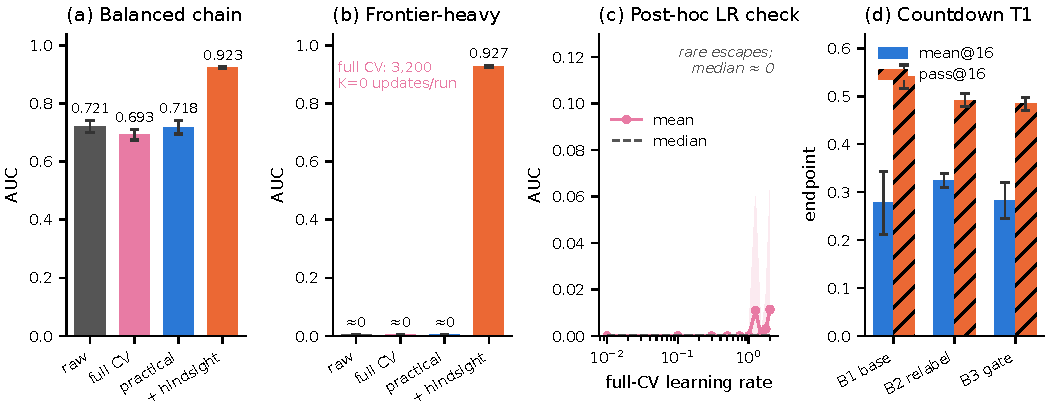
\includegraphics[width=\linewidth]{figures/fig2_ladder}
\caption{\textbf{The ladder.} (a) Exact-gradient chains: a no-floor,
$\gamma$-matched true-pass-rate oracle matches the full stack within
the observed five-seed variation --- allocation saturates --- and
recycling still adds on top of the oracle. (b) Frontier-heavy regime: allocation scores exactly zero;
recycling solves it, and does so equally under uniform sampling
(.931 vs.\ .928) --- creation, not allocation, is the live channel.
(c) Maze at matched wall-clock: 3/3 seeds on both meters. (d) The
original GSM8K $2{\times}2$ is shown only as treatment-delivery
diagnosis: one GRPO+teacher seed regressed and one did not, while
posterior steering remained weak; the subsequent controlled cell
missed its pre-registered delivery gate and is inconclusive
(\S 6.7).}
\label{fig:ladder}
\end{figure}

\paragraph{6.1 Does allocation saturate? (exact-gradient skill chains; CPU, 5 seeds).} Uniform 0.650
$\to$ teacher 0.728 $\to$ full stack $\mathbf{0.890 \pm 0.002}$ AUC
(Fig.~\ref{fig:ladder}a). An
eight-arm control battery (App.~\ref{app:rungs}) orders into a
\emph{gradient-information ladder}, each rung a 5/5 paired-seed win:
zero-information dose ($0.798$--$0.800$) $<$ replayed correct direction
($0.832$) $<$ true relabels ($0.869$) $<$ perfect allocation (oracle
$0.8885 \approx$ full stack $0.8895$) $<$ allocation$+$creation
($0.8935$). Two decompositions matter downstream. \emph{Allocation
saturates at the top of the ladder, not at the teacher}: a no-floor,
$\gamma$-matched true-pass-rate oracle ($0.8885{\pm}.0014$) sits
within the five-seed variation of the \emph{full stack}
($0.8895{\pm}.0023$) --- similar within observed noise, not tested for
equivalence. The posterior-only teacher scores $0.728$, far below the
oracle, so perfect difficulty information is worth a great deal over
the posterior alone; the accurate reading is that \emph{recycling
compensates for the posterior's allocation error} --- the combination
reaches what perfect information reaches, by a different route. \emph{Creation decomposes}: a replay
placebo captures 83\% of recycling's $+0.22$; the relabel
\emph{direction} carries $+0.037$ beyond it and is the most reliable
arm in the battery, while random-target relabels lose to dose-matched
replay 5/5. The utility form matters through its $N$: the
$N$-blind learnability slice $p(1{-}p)$ forfeits the entire allocation
gain at $N{=}16$ ($-.007$ vs.\ uniform) where $u_N$ carries $+.078$
(5/5). A post-guidance exploratory fixed-completion sweep then held
51{,}200 sampled completions per cell across
$N\in\{2,4,8,16,32\}$ (8 paired seeds, MaxRL estimator, no
recycling). As required algebraically, $u_2=p(1-p)$ produced identical
trajectories. For every $N>2$, $u_N$ beat $p(1-p)$ in 8/8 paired
seeds, with mean AUC differences $+.0307,+.0920,+.1526,+.1909$ as
$N$ increased. Against uniform, however, $u_N$ was slightly worse at
$N=2,4$ and better at $N=8,16,32$: evidence for rollout awareness,
not a blanket curriculum advantage (structured artifact
\texttt{results\_fixed\_budget\_n\_sweep.json}). In the original
$N{=}16$ battery all arms converge within $.027$ of one another --- on fixed pools these
interventions buy \emph{time-to-ceiling}, not the ceiling.
\takeaway{A monotone information ladder: dose $<$ direction $<$
allocation-ceiling $<$ +creation. Allocation saturates; creation adds
on top; every intervention buys speed, not asymptote.}

\paragraph{6.2 Can any sampler act when nothing is learnable? (frontier-heavy regime, max pool pass rate $10^{-5}$; 5 seeds, artifact committed).}
Uniform, DAPO, and the plain teacher score \textbf{exactly 0.00};
adding recycling reaches \textbf{0.98 final (0.93 AUC)} --- relabeling
invents the curriculum below the pool, ignites within ${\sim}400$
groups, then goes silent. The attribution control pins down which
channel did it: \emph{uniform}+recycling scores the same
($0.931{\pm}.002$ vs.\ teacher+recycling $0.928{\pm}.003$ AUC) --- in
this regime the entire effect is signal creation; allocation
contributes nothing because there is nothing learnable to allocate
toward. Equivalently: a designer who hand-added the achieved sub-goals
to the pool would also escape the zero --- what recycling buys is
\emph{discovering} that sub-pool from the policy's own failures, with
no task engineering. The one loss-level alternative --- the full
control-variate estimator, which is \emph{not} silent at $K{=}0$ ---
also scores $0.000$ in every seed on this pool despite spending 100\%
of its update norm on all-fail groups: the all-fail term pushes every
sampled action down symmetrically and cannot ignite a pool this deep
(5 seeds, matched budget; artifact
\texttt{results\_fullcv\_baseline.json}; detail in
App.~\ref{app:rungs}).
\takeaway{Where nothing is learnable at budget, sampling policy is
irrelevant --- uniform and teacher tie at zero without recycling and
tie at 0.93 with it. Even the estimator family's nonzero all-fail
update (full control variate) stays at zero here: creation is the
only channel we tested that ignites a dead pool, and its value is
discovery, not allocation.}

\paragraph{6.3a Does the curriculum pay on the maze? (transformer at
matched wall-clock; 1.26M params, 13 levels, 3 seeds).} Champion
(teacher + dense recycling) $0.252{\pm}0.005$ final /
$0.229{\pm}0.009$ AUC vs.\ uniform $0.230{\pm}0.015$ /
$0.211{\pm}0.011$; paired deltas positive in 3/3 seeds on both meters
(six correlated contrasts, not six seeds); 22--35\% more optimization
steps per GPU-hour. Attribution: matched \emph{wall-clock} lets
curriculum arms take $1.2$--$1.4\times$ more optimization steps (dead
groups skip the backward pass), and step-matched truncation shows the
extra steps are most of the pure teacher's effect (step-matched
teacher-only $\Delta$AUC $+0.006$, within seed noise) while
teacher+recycling survives step-matching, positive in all three paired
seed blocks\footnote{A paired $t$ at $n{=}3$ gives $p{\approx}.04$,
reported as descriptive given its normality sensitivity; an exact
sign-flip test cannot go below $.25$ at three blocks.} --- on the maze
the teacher's measured value is \emph{throughput}, recycling's is
signal. Utility-form controls (3-seed reruns, artifact
\texttt{un\_form\_verdicts.json}): the exact $u_N$ measures within
noise of the legacy deployed form on the maze itself, and a
CPU-winning $(1{-}p)$-tilted refinement loses 0/3 here --- within-band
utility choices are testbed-sensitive, which is why the theory claims
only the band's boundaries.

\paragraph{6.3b Does the estimator effect survive real gradients?
(the pre-registered factorial).} An earlier
nine-run cohort showed perfect sign separation --- every MaxRL-labeled
run grew $\passat{8}$, every GRPO-labeled run lost it --- but the pool
mixed sampler configurations and hindsight doses and reused
warmstarts, so we pre-registered the clean test: a balanced
$\{$MaxRL, GRPO$\}\times\{$uniform, $u_N$-teacher$\}$ factorial, six
independent seed blocks, identical per-block warmstarts, matched
generation-and-optimization budgets (250 fixed steps), one registered
endpoint (paired $\Delta$ mean $\passat{8}$, final minus warmstart),
and a committed falsification branch. \textbf{The endpoint failed:
3/6 paired blocks under uniform, 4/6 under the teacher, and only 4/12
MaxRL cells grew coverage at all --- the cohort's zero-exception
divergence is retracted, not softened} (prereg + raw cells + verdict:
\texttt{curriculum\_maxrl/maze\_gpu\_factorial/}, vendored with
execution-commit provenance). The cohort pattern had conflated
recycling's coverage contribution with the estimator effect: its MaxRL
runs included hindsight arms, and the factorial isolates the
estimator.

\subparagraph{What survives, at its evidence level.}
\emph{Confirmed, exact rung --- at matched learning rate}: frozen
realized schedules replayed under each estimator preserve MaxRL over
GRPO in 10/10 seed$\times$schedule pairs at the common deployed lr
(artifact \texttt{results\_schedule\_matched.json}). A pre-registered
lr sweep then tested whether this is an lr-calibration artifact
(reviewer-posed; P-LR1 --- falsified as registered, branch
executed), and on this learnable-everywhere pool it partly is: a global $2$--$4\times$ lr
raise lets GRPO match MaxRL's $\Delta$cov@8 --- by saturating
$\passat{1}$, so its coverage--reliability premium collapses to
$.007$--$.013$ where MaxRL holds $.050$ (artifact
\texttt{results\_lr\_matched.json}). Per the committed branch we
state the exact-rung ordering as an at-matched-lr fact and carry the
normalization caveat as a limitation: on pools where everything is
learnable, more learning of any kind buys coverage, and only the
premium separates the estimators; the neural-scale claim (below) is
the one tested at matched budgets \emph{and} identical optimizer
settings --- and its premium version also holds there (exploratory,
computed after the lr sweep identified the premium as the invariant
currency: both sampler contrasts are positive within each of 12
independent seed blocks across the two waves; the two sampler
contrasts are repeated observations within block, not 24 replicates;
artifact
\texttt{premium\_reanalysis.json}). \emph{Found exploratorily; according to the
external execution record, specified before a fresh wave}: on time-integrated coverage (mean
in-training $\passat{8}$ minus warmstart), MaxRL retains more coverage
than GRPO under both samplers in all six wave-1 seed blocks --- a
noise-integrating secondary not specified for wave 1. The external record says
it became the primary of a fresh six-block wave (P-F2, $\ge$5/6 under both
samplers) and met that rule at 6/6 under each sampler (exact two-sided sign
$p{=}0.031$ per sampler; means
$+.015$/$+.024$). Averaging the two correlated sampler contrasts
within each wave-2 block gives mean $+0.01950$ and a post-hoc 95\%
t interval $[+0.01148,+0.02752]$; across both waves all 12
block-averaged contrasts are positive (descriptive mean $+0.02175$,
95\% interval $[+0.01663,+0.02688]$; no pooled confirmatory
$p$-value). P-F3 met its pre-registered pair-level bar at 10/12, but
those pairs are correlated within seed. After block averaging, four
contrasts are positive, one is tied, and one is negative, with
interval $[-0.00330,+0.16996]$. We therefore treat easy-band
localization as suggestive rather than established. The retired \emph{endpoint}
contrast, unregistered on the fresh blocks, landed 5/6 there ---
consistent with the power analysis (\S\ref{sec:limits}) and left
retired; the claim this paper makes is the time-integrated one.

\begin{figure}[t]
\centering
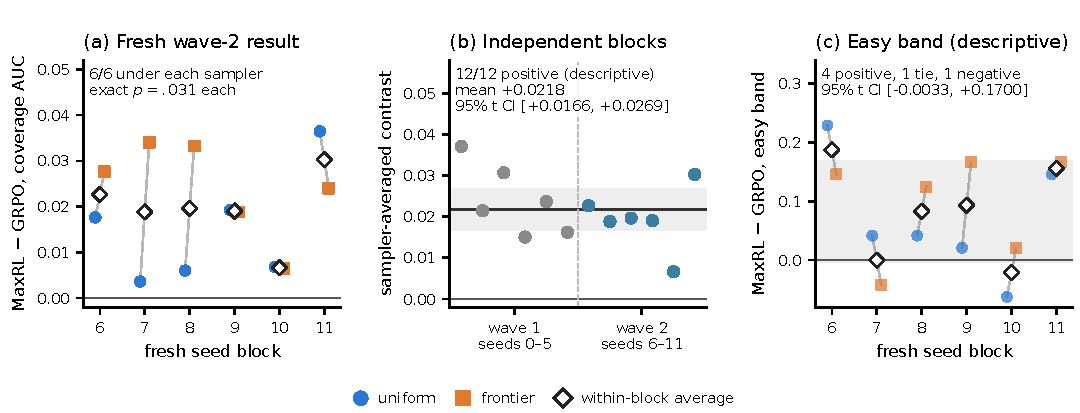
\includegraphics[width=\linewidth]{figures/fig_maze_block_contrasts}
\caption{\textbf{Balanced maze factorial at the independent seed-block
unit.} \emph{(a)} Wave 2 confirms the registered time-integrated
coverage ordering in 6/6 blocks under each sampler; connected sampler
contrasts share a seed/warmstart and are repeated observations, with
the diamond their within-block average. \emph{(b)} The sampler-averaged
contrast is positive in all 12 independent blocks across waves
(descriptive across the exploratory and confirmation waves; no pooled
confirmatory $p$-value). \emph{(c)} The registered pair-level
easy-band bar was met, but block averaging gives four positive, one
tie, one negative, and an interval including zero, so localization is
suggestive.}
\label{fig:blockfactorial}
\end{figure}

\subparagraph{Three controls close alternative readings.}
\emph{Scheduler mismatch}: GRPO driven by its \emph{own} exact mass
functional ($\frac1N\mathbb{E}\sqrt{K(N{-}K)}$, Thompson-sampled) does
not close the gap on chains (5/5) and loses coverage like every other
GRPO arm in the factorial (5/6 cells negative, mean $-.042$, equal to
uniform-GRPO) --- no scheduler choice rescues the estimator.
\emph{Variance normalization}: on chains, removing GRPO's SD
normalization drops it to RLOO's coverage profile exactly as the mass
account predicts ($.148$ vs.\ RLOO $.161$; sample-SD $.762$) --- but
in the factorial the no-SD arm loses the easy band in 6/6 seeds,
indistinguishable from sample-SD GRPO, so \textbf{at neural scale the
easy-band liquidation is not explained by variance normalization
alone}: the Fig.~\ref{fig:utility} mechanism holds per-task under
exact gradients and does not transfer through shared parameters
unmodified (committed revision, falsification branch P-G0c).
\emph{Interaction}: the teacher does not amplify GRPO's coverage loss
in the factorial (teacher$-$uniform $\Delta$cov@8 under GRPO: mean
$+.015$, mildly protective) --- the GSM8K P-G2 regression pattern
receives no corroboration from the maze at this budget. Inference
currency (single checkpoint pair; convention and per-level detail in
App.~\ref{app:rungs}): our checkpoint needs $\mathbf{11\times}$ fewer
samples at level 5, ties GRPO at levels 2--3 --- the summed-coverage
curves cross at $k{\approx}4$, so choose the estimator by how many
samples you will draw at inference.

\paragraph{6.4 Where and when does GRPO's coverage go? (level-resolved;
cohort data --- read with \S 6.3b's retraction).}
This section decomposes the \emph{original heterogeneous cohort} by
difficulty band; after the factorials, its value is a hypothesis about
the location and timing of GRPO's loss (wave 1: 9/12 exploratory
pair-level contrasts; wave 2 P-F3: registered bar met at 10/12
pair-level contrasts, but only 4/6 positive after block averaging,
with one tie, one negative, and an interval including zero), not
the retired zero-exception contrast (Fig.~\ref{fig:bands}). \emph{Where:} GRPO's $\passat{8}$
loss is concentrated almost entirely on the easy/mid band L1--3
($-.224$ mean over its four runs, every run negative) while its L1--3
$\passat{1}$ \emph{rises} ($+.02$ to $+.14$, every run) --- it funds
reliability by liquidating easy-band coverage; MaxRL holds L1--3 flat
($+.005{\pm}.058$ over 18 runs) and concentrates its gain on the
frontier band L4--6 ($+.126{\pm}.063$ vs.\ GRPO's $+.057$). The
18-run MaxRL pool is a heterogeneous run inventory (teacher variants,
hindsight doses, a wide model, repeated seeds), so we report the band
asymmetry descriptively --- every GRPO run negative on L1--3, the
MaxRL spread centered at zero there --- and attach no permutation
$p$-value; the 22 runs are not exchangeable replicates of one
estimator contrast. This is consistent with the mass curves in Fig.~\ref{fig:utility} ---
the $\sqrt{K(N{-}K)}$ weighting keeps spending updates on mastered
prompts where $u_N$ has already released them --- but the step from
mass to coverage is a stated \emph{hypothesis}, not a derivation: mass
is sign-blind, and ``mastered-tail updates sharpen'' requires an
argument about the sign structure of near-saturated groups that we
support with the location and timing evidence here rather than prove.
Its committed falsifier (remove variance normalization and the tail
signature should vanish) split across the rungs, as \S 6.3b reports:
the mechanism account is per-task-exact only, and we bound the claim
accordingly.
\emph{When:} the divergence is immediate, not saturation-triggered ---
GRPO incurs 59--73\% of its total coverage--reliability gap loss
($\overline{\passat{8}-\passat{1}}$: $.123\to.042$) within the first
quarter of the budget, with the first easy-band $\passat{8}$ drop
visible at steps 0--50 when L1 $\passat{1}$ is still only $.62$--$.75$;
MaxRL's premium stabilizes after warmup ($.122\to.101$). A
dose-response note from the same logs (descriptive, same caveat as
above): sparse relabeling (1/dead group) uniquely preserves the
coverage--reliability gap ($\overline{\passat{8}-\passat{1}}$) relative to none and dense, while dense banks the
same coverage into the best final $\passat{1}$ --- dose sets
\emph{where} the coverage dividend is spent, not whether coverage is
lost.

\begin{figure}[t]
\centering
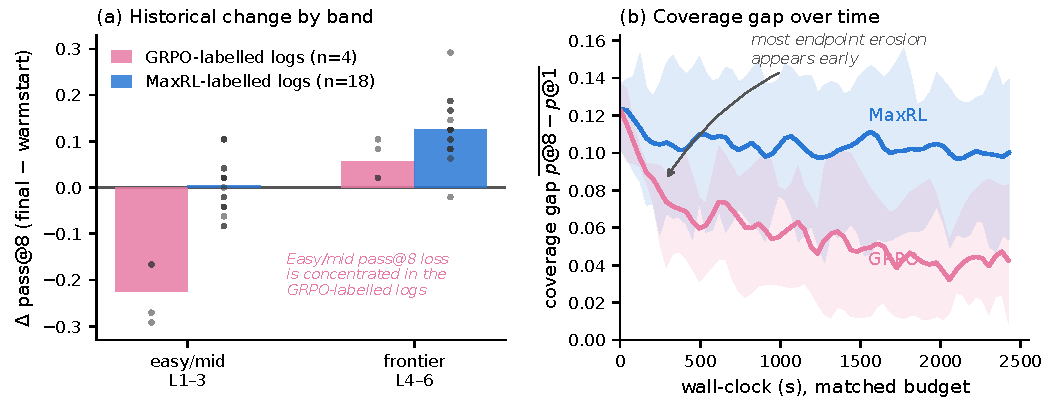
\includegraphics[width=\linewidth]{figures/fig8_bands}
\caption{\textbf{Where and when GRPO's coverage goes (maze,
level-resolved, matched wall-clock).} \emph{(a)} $\Delta \passat{8}$
(final $-$ warmstart) by difficulty band: GRPO's loss lives on the
easy/mid band (all 4 runs; dots are runs) while its $\passat{1}$ there
rises --- sharpening; MaxRL holds the easy band and gains on the
frontier band (18 runs; a heterogeneous run inventory --- descriptive,
no $p$-value). \emph{(b)} Coverage--reliability gap
$\overline{\passat{8}-\passat{1}}$ vs.\ wall-clock (mean and min--max
across runs): GRPO's erosion begins within the first ${\sim}25$--$50$
steps, before any level saturates; MaxRL stabilizes after warmup.}
\label{fig:bands}
\end{figure}
\takeaway{The heterogeneous cohort localizes GRPO's loss to the easy
band, and the factorials show the same direction in most within-block
sampler contrasts. However, wave 2 has only four positive block
averages, one tie, one negative, and an interval including zero, so
localization remains suggestive; the variance-normalization mechanism
holds only at the exact rung.}

\paragraph{6.5--6.6 Two boundary rungs (compressed; full protocols,
figures, and attribution in App.~\ref{app:rungs}).} An IsaacLab
Anymal-C pilot (5 arms, one seed, independent team, pre-registered
null) marks where allocation does \emph{not} pay: on a terrain grid
learnable everywhere at budget, the stock greedy curriculum beats the
frontier teacher outright (.372 vs.\ .278) --- with the maze
step-matched analysis and Countdown, the regime pattern is
\textbf{allocation pays where unlearnable-at-budget regions exist to
avoid}. A Gymnasium control suite (binary task success, 3 seeds)
marks the opposite boundary: training on the target task alone is a
provable zero-update freeze (every group all-fail, so every
group-relative estimator emits exactly zero), while the gated full
stack reaches $1.000{\pm}0.000$ on both official tasks
(Fig.~\ref{fig:gym}, appendix); attribution
shows task spread supplies gradient existence, the teacher speed and
stability, and a per-bin-parameters ablation reproduces the known
failure --- \textbf{curricula operate through shared parameters, or
not at all}.

\paragraph{6.7 Was the LLM-scale curriculum treatment delivered?
(GSM8K; pre-registered; SmolLM2-360M, $N{=}16$).}
The original $2{\times}2$ produced a regression shape in one of two
GRPO+teacher seeds, while posterior starvation kept every teacher
cell close to uniform. We therefore pre-registered a
steering-controlled cell with a treatment-delivery gate: minimum
dead-sampled fraction $<0.50$ and run mean $<0.60$. The completed
50-step cell reached minimum $0.413$ but run mean $0.601480$, missing
the mean gate by $0.00148$ (final mean@4 $0.10547$;
$\passat{4}=0.19834$). Under the committed decision rule, this is
\textbf{inconclusive by design}: the intended steering treatment was
not reliably delivered, so its endpoint is evidence neither for nor
against an estimator--teacher interaction. We retain GSM8K only as a
treatment-delivery negative and require a short pilot to clear the
gate before any new full cell.
\takeaway{At this pool size and budget, prompt-level posterior
steering starved before it became a testable neural treatment.}

\begin{figure}[t]
\centering
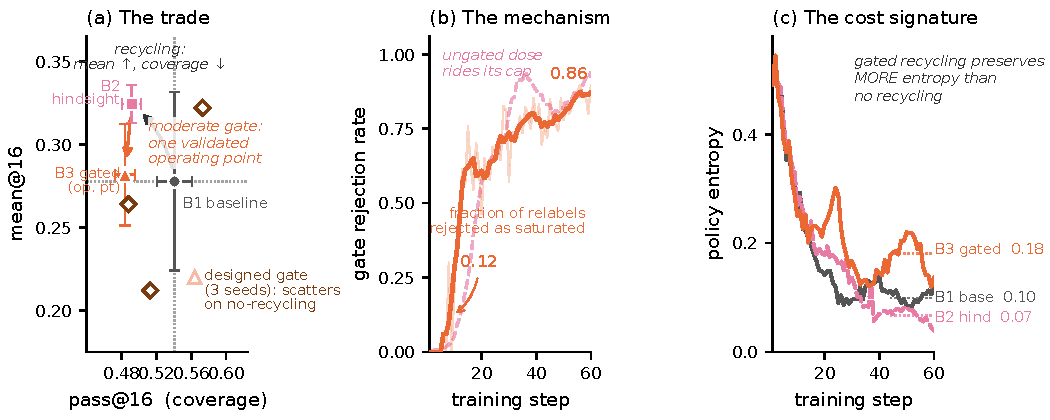
\includegraphics[width=\linewidth]{figures/fig7_sharpening}
\caption{\textbf{Recycling-package concentration and a secondary
saturation-gate study (Countdown, tier 1).} \emph{(a)} Three-seed
aggregates: recycling (B2) raises mean@16 while the logged VERL bootstrap
best@16 coverage proxy falls; the original under-gated B3 setting gives most
of the mean back on this early-saturating tier but used faulty decay
math. The externally specified corrected-code designed-strength arm
(diamonds; 3 seeds, corrected decay, rejection ${\sim}.94$) refuted
the strength-dial reading: its seeds scatter around the no-recycling
point rather than extending a frontier (P-R1, \S 6.9), so it is drawn
as a scatter per the committed falsification branch; the superseded
1-seed point (faint) sits inside that spread. \emph{(b)} Descriptive gate
telemetry: the rejection rate rises over training, consistent with but not
identifying destination saturation, while the ungated dose rides its cap.
\emph{(c)}
The faulty-decay gated arm ends with more policy entropy than no recycling;
this is descriptive telemetry, not a validated operating point.}
\label{fig:sharpening}
\end{figure}

\paragraph{6.8 Historical Countdown development result (superseded).}
The original $2{\times}2$ exact-verifier experiment returned two null
predictions because its pool had little headroom. Its single-run concentration
pattern motivated the rebuilt three-seed study below, but it is not the applied
claim. The metric originally labeled pass@16 is VERL bootstrap best@16 and must
be read as a coverage proxy under the erratum above.

An externally specified higher-dose arm later applied two optimizer epochs to
every live group with hindsight disabled. It reached mean@16
$.478{\pm}.021$ and bootstrap best@16 $.635{\pm}.046$. Recycling permits at
most 12 auxiliary groups per 64 requested groups, whereas this replay arm
doubles epochs on every live group. It is therefore a higher-dose alternative
that improves both logged metrics, not a dose-matched control, relabel-specific
effect, or causal bound. Complete relabel-arm seed records and per-task outcomes
remain missing.
\takeaway{The original pool is a development null. The higher-dose replay arm
does not identify the effect of relabel direction.}

\paragraph{6.9 Does the gate recover it? (Countdown v2 pool, 3
seeds, pre-registered).}
\emph{The gate, and what it is not.} The rule we implement is a
saturation heuristic: a decayed frequency statistic $\hat f_{g'}$ over
the recycler's own recent relabel destinations, thresholded at
\texttt{gate\_max\_p}. It is \emph{not} an estimate of the destination
task's fresh-rollout pass rate $p_\theta(\text{success} \mid g')$ ---
the gate never rolls out $g'$ and never observes a $g'$ failure ---
and the threshold $0.5$ is a tuned midpoint, not a derived
zero.\footnote{$u_N$'s exact high-$p$ zero is at $p{=}1$, which would
admit everything; a gate on a genuine task-conditioned $\hat p_{g'}$
is the derived object.} Where destination pass rates are exactly
measurable (skill chains, 10 paired seeds; artifact
\texttt{results\_gate\_variants.json}), the true-$p$ gate preserves
essentially all of ungated recycling's value (AUC $.879$ vs.\ $.881$)
while the frequency heuristic pays a toll ($.798$; 10/10); at decision
time the heuristic's statistic \emph{anti-correlates} with true
$p(g')$ ($-.27$ --- it tracks the recycler's own recent output), and
the two rules agree only once everything saturates ($.66 \to .99$).
The results below are therefore evidence about a recency-novelty
filter that approximates saturation late in training. The upgrade is
also practical, not just derived: an \emph{estimated}-$p$ gate fed by
probe rollouts of proposed destinations recovers $98\%$ of the
oracle-vs-frequency gap at matched \emph{total} rollouts with even
one probe per step (10/10 seeds at every probe budget tested,
insensitive to the budget over $1$--$16$; pre-registered P-PB1,
confirmed; artifact \texttt{results\_gate\_probe\_budget.json}) --- destination
pass rates are cheap to estimate because the gate only needs them
coarsely ($\lessgtr 0.5$), so the LLM-loop version costs a
negligible slice of generation budget.

\emph{The experiment.} We rebuilt the pool with real structure
(random operand permutation, parenthesization, exact division; a
headroom gate excluded guesser-saturated tiers) and ran three arms
$\times$ three seeds: no recycling (B1), ungated recycling (B2), gated
recycling (B3). One setup note kept for its theory reading: recycling
has a \emph{syntactic prerequisite} --- the pre-SFT base model
produces zero verifier-valid failures, so there is nothing to recycle
until SFT installs the output format (pool construction and baseline
calibration in App.~\ref{app:rungs}). \textbf{Aggregate concentration
pattern:} at tier 1, recycling raises mean@16 by $+.046$
($.278{\pm}.066 \to .324{\pm}.014$) while VERL bootstrap best@16
falls by $-.049$ ($.541{\pm}.024 \to .492{\pm}.013$), reported as
mean $\pm$ sample SD across three seeds. Complete B1/B2 records are
not vendored (seed 3 is aggregate-only), so we do not claim paired
seed signs. Figure~\ref{fig:passk} shows seed 1's exploratory logged
proxy over $k$; per-task outcomes are unavailable and standard
unbiased pass@$k$ cannot be reconstructed.

\begin{figure}[t]
\centering
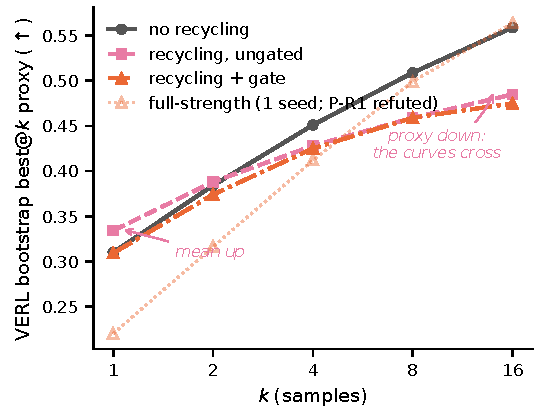
\includegraphics[width=0.52\linewidth]{figures/fig9_passk}
\caption{\textbf{Exploratory single-seed VERL bootstrap best@$k$ proxy
(Countdown tier 1, step-60 val, $n{=}128$ tasks).}
This with-replacement metric is not standard unbiased pass@$k$. Ungated
recycling sits above baseline at $k{=}1$ and below by $k{=}4$ in the
logged proxy, with the deficit widening with $k$. The
moderate gate tracks baseline at low $k$ with a smaller high-$k$
deficit; the full-strength curve (hollow; one seed, corrected decay)
pays at $k{=}1$ and finishes above baseline at $k{=}16$, but the
strength-dial reading this suggests was refuted in the 3-seed
designed-strength sweep (P-R1, \S 6.9). The single-seed points and
session provenance are stored in the declared figure input; they are
exploratory and cannot be converted without the underlying task outcomes.}
\label{fig:passk}
\end{figure}
Available aggregate dynamics suggest that the mean increase precedes the
proxy decrease, but complete seed-level records are absent. We therefore do
not make paired timing, per-seed direction, or early-stopping claims.

\textbf{The gate did not validate.} The favorable moderate-gate setting used
faulty decay code and remains descriptive. A corrected, externally specified
strong-gate sweep landed near the no-recycling aggregate and refuted the
claimed monotone gate dial; it does not establish equivalence. Rejection and
entropy telemetry are consistent with saturation filtering but do not identify
the cause of the aggregate pattern. A successful, fixed-code mitigation
remains open.
\takeaway{The retained result is mean-up with a bootstrap coverage proxy down.
The gate and the causal concentration mechanism are not validated.}

\section{Related work}
\textbf{The coverage tension.} RLVR itself trades coverage for precision:
$\passat{1}$ rises while $\passat{k}$ at large $k$ falls below the base
model \citep{yue}, with entropy collapse as the mechanistic signature
\citep{cui} and overtraining on saturated problems as a locus
\citep{yuan}. Our contribution to this line is the \emph{interaction}:
whether external curricula and recyclers compound or cancel the
estimator's implicit weighting, and what that costs in coverage. Notably,
recent work frames curricula as the \emph{cure} for coverage loss
\citep{cai}; our GRPO arms show the cure is estimator-conditional ---
those studies never varied the estimator. The estimator--difficulty
interaction itself is a heating 2026 theme --- SC-SDPO \citep{scsdpo}
shows GRPO's normalization implicitly encodes a difficulty weighting,
and A-GRAE \citep{agrae} redesigns the advantage around difficulty
focus --- but to our knowledge no prior work runs \emph{identical}
curricula under two estimators or measures the resulting
$\passat{k}$ coverage ordering.

\textbf{Curricula for RLVR.} Difficulty-adaptive sampling is bucket- or
scalar-level and heuristic-scored: DUMP (UCB over buckets), AdaRFT
(scalar controller over precomputed labels, TMLR 2026), SEC (category
bandit), threshold curricula. ProCuRL \citep{procurl} is the closest
mathematical predecessor: with target success one, its proximal score
is $p(1-p)=u_2(p)$. SFL \citep{sfl} and LILO \citep{lilo} likewise
prioritize binary reward variance. Our separate paid-probe comparison
implements ProCuRL's environment-selection semantics on the common Acrobot
learner; at the frozen refresh cadence, probe accounting overwhelms score
differences. Our novelty claim is therefore not
the intermediate-difficulty rule, but the arbitrary-$N$ functional
derived from the practical MaxRL estimator, its $N{-}1$ correction,
and an estimator-by-sampler coverage test. SPEED \citep{speed} uses a
probe-and-band rule justified by gradient-estimator SNR, while VCRL
\citep{vcrl} thresholds realized group variance with memory; these are
the direct RLVR baselines that a full fixed-budget comparison must
include. Classical
PLR \citep{plr} prioritizes future learning potential using TD error
and staleness, while ALP-GMM \citep{alpgmm} uses temporal absolute
learning progress. Those scores can react to forgetting; coefficient
mass is instead an instantaneous estimator-matched activity proxy.
Reinforce-Ada \citep{reinforceada} --- the adaptive
sampler MaxRL itself points to --- adapts the rollout count \emph{within}
a prompt until a signal criterion is met, holding the prompt distribution
fixed; our teacher is the complementary move, reallocating \emph{across}
prompts at fixed group size, and the static water-filling reference
(App.~\ref{app:alloc}) is the idealized form of both. DAPO's dynamic sampling and
GRESO cull dead prompts --- avoidance without allocation or creation.
PKPO \citep{pkpo} and Pass@$k$ training \citep{passk}
modify the objective toward $\passat{k}$ but keep uniform sampling.

\textbf{Finite-rollout objectives and adaptive allocation.}
RL2ML \citep{rl2ml} separates population objectives from group-level
update scale and gives exact finite-rollout variance and metric-gain
analyses. It makes the scope boundary important: our coefficient mass
is neither update norm, gradient direction, variance, nor expected
metric improvement. DARS \citep{dars} adaptively deepens rollouts on
hard prompts and studies pass@$K$; it allocates rollout count within a
prompt, whereas FrontierMax changes cross-prompt sampling probability
at fixed $N$. These concurrent lines motivate the fixed-total-rollout
$N$-sweep and matched-update analyses in our release plan.
\textbf{Goal selection in HER.} Selecting \emph{which} goals to
train on by difficulty or reachability is a decade-old idea in the
relabeling literature: intermediate-difficulty goal generation
\citep{goalgan}, value-based hindsight goal selection (HGG;
\citealp{hgg}), curriculum-guided HER's proximity--diversity admission
of relabel goals \citep{cher}, and Skew-Fit's $\alpha$ as a
concentration-vs-coverage dial \citep{skewfit}. Our gate belongs to
this mechanism class; what is new is not admission-by-difficulty but
its \emph{motivation} --- the same estimator functional $u_N$ that
schedules sampling says mastered-tail updates carry no fresh signal,
so the teacher and the gate answer to one object --- and the coverage
accounting used to evaluate it. The gate statistic itself is a
tuned heuristic (a decayed achieved-destination frequency with a
tuned threshold, \S 6.8--6.9), so we claim a shared motivation, not a
switch-free derivation.

\textbf{Hindsight and self-training for LLMs.} Exact-verifier
relabeling has precedent outside RLVR loops --- CodeIt \citep{codeit}
(ARC program synthesis, relabel + prioritized replay) and proof-tree
relabeling \citep{minimo} --- and LLM-judged variants relabel agent
trajectories (AgentHER, HSL). Concurrent 2026 work brings
relabeling-adjacent mechanisms into RLVR-style training: LfH \citep{lfh}
(a VLM proposes one shared hindsight instruction per failed group for
VLA post-training; the relabeler is a judge, their stated limitation)
and ZipRL's hindsight response replay \citep{ziprl} (densifying GRPO
signal for multi-turn agents). These works motivate studying diversity under
relabeling, but our retained Countdown scalar is only a bootstrap best@$k$
proxy and cannot establish a standard pass@$k$ cost. We therefore make no
priority claim for that pattern. The narrow distinctions retained are the
arbitrary-$N$ expected half-mass of the deployed practical-MaxRL convention,
its $T=N-1$ all-fail handling, and the estimator-by-sampler maze coverage
factorial. The proposed relabel-admission gate failed its fixed-code strong
test and is not a contribution.

\section{Limitations and negative results}\label{sec:limits}

\paragraph{Scale, and what the retraction taught about design.} The
factorial retraction is reported in full in \S 6.3b. The registered endpoint
failed; time-integrated coverage was then selected exploratorily and, according
to the external execution record, specified before a fresh six-block wave.
That wave is positive 6/6 under each sampler, with sampler-averaged mean
$+.0195$ and post-hoc interval $[+.0115,+.0275]$. Raw checkpoint trajectories
are absent, so the frozen AUC multiverse cannot yet test sensitivity to warmup,
horizon, and integration choices. The original LLM-scale
teacher$\times$estimator pattern appeared in one of two seeds and was
not corroborated by the maze factorial. More importantly, the
subsequent steering-controlled GSM8K cell missed its pre-registered
treatment-delivery gate: minimum dead-sampled fraction $0.413$ passed
the $<0.50$ condition, but run mean $0.601480$ missed the $<0.60$
condition by $0.00148$. Per the committed branch, the cell is
inconclusive by design and its endpoint is not evidence for or against
the interaction. No additional full cell is warranted until a short
pilot demonstrates treatment delivery.

\paragraph{Paid probing can erase the allocation budget.}
The separate 80-pair Acrobot comparison is a source-faithful
selection-semantic comparison on the common 640-parameter practical-MaxRL
learner, not a reproduction of ProCuRL's complete PPO system. Its frozen
5,120-student-transition refresh cadence charges every probe transition and
spends about 93.2\% of paid transitions on probes. The resulting null between
$u_{16}$ and ProCuRL selection and the roughly $.31$ AUC deficit of every
probed arm versus ordinary uniform support a cadence-specific probe-cost
diagnosis for this learner, not general ProCuRL inferiority or performance
under a cheaper probe design. Its local source/runtime lock is mechanical
provenance but has no immutable public pre-execution commit.

\paragraph{Where the teacher cannot work as specified.} Two structural
limits at production scale, stated as design constraints rather than
future work. \emph{Posterior starvation is the generic regime}: a
per-prompt Beta posterior needs multiple visits, but realistic RLVR
pools see ${\sim}1$ epoch (${\le}2$--3 visits per prompt), so
FrontierMax as specified is a small-pool instrument; deploying it on
$10^5$-prompt pools requires coarser state --- bucket-level posteriors,
a learned difficulty predictor, or warm starts --- and our external
annotations transferred poorly ($\rho{=}-0.17$), so cold-start from
off-model labels is not the answer. \emph{The throughput mechanism
does not transfer}: at matched wall-clock the maze teacher's measured
value is extra optimization steps from skipping dead groups' backward
passes, but in generation-dominated LLM pipelines (up to 83\% of step
time in our generation-dominated sessions; App.~\ref{app:hparams})
a dead group has paid its full cost before it is known dead --- the
relevant LLM-scale comparisons are generation-budget-matched
(resample-to-fill, prompt pre-filtering), and the teacher's value
there rests on avoiding the generation itself, which requires the
posterior it starves for. These two constraints compound, and we state
them together because they bound the same deployment.

\paragraph{Scope of the surrogate.} Coefficient mass is not gradient
norm, SNR, or expected improvement (Remark~\ref{rem:scope}) --- it
omits score-vector geometry, sequence length, token masking, optimizer
state, and clipping --- and \S 6.5
exhibits the regime where reallocating it buys nothing
(learnable-everywhere pools). Recycled-gradient exactness is a property
of the environment's relabel map; noisier verifiers will land between
our fixed-pool and one-shot endpoints ($+0.22$ vs.\ $+0.01$ AUC).

\paragraph{The coverage main effect is pool-conditional.} A
pre-registered fifth suite (Jugs water-measuring puzzles;
preregistration, per-cell raw endpoints, verdicts, and postmortem
vendored under \texttt{jugs\_llm/results/} with execution-commit
provenance) returned all-null: on a pool whose
learnable band is a single stratum of 1--2-move template solutions,
\emph{plain MaxRL} also collapses --- entropy $1.36 \to 0.07$--$0.21$
in 60 steps, frontier-tier $\passat{16}$ $0.15 \to 0$, every arm
converging to the same deterministic policy --- and recycling
accelerates the collapse rather than rescuing it. When $N$ rollouts of
a near-trivial plan are near-identical, the i.i.d.-rollout diversity
the group contrast requires is absent, and success-conditioned weights
liquidate frontier coverage through shared parameters just as GRPO's
do elsewhere. The estimator main effect of \S 6.3--6.4 is therefore a
claim about pools with a graded band at the deployed $N$, not an
unconditional safety guarantee; per-task rollout-set diversity at
initialization is the design gate we now check first. The same suite
also exposed a granularity bug in the gate (keying destinations by
value collides tasks when achieved values are few and shared ---
$\le 20$ integers in Jugs vs.\ hundreds in Countdown); the corrected
gate keys on the relabeled task.

\paragraph{What did not transfer.} A $4\times$ duration run refuted
our own duration hypothesis (the deep-frontier stall is a
per-step-competence ceiling; depth needs capacity, not schedule);
$\gamma$-concentration did not transfer from chains to the maze,
as the compounding model predicted; adaptive truncation order
underperformed fixed $T$; and feeding relabeled successes to the
teacher's posterior inflates it, so the posterior sees requested-task
evidence only.

\paragraph{Corrections along the way.} Two early claims were retracted
on internal review --- a teacher-steering read traced to an
epoch-frozen sampler (the fixed run confirmed the effect), and a
``beats the oracle'' comparison traced to a floor handicap in the
oracle arm (\S 6.1 reports the corrected match-within-noise). Full
postmortems live in the repository's audit trail.

\section{Conclusion}

For the practical success-conditioned estimator under i.i.d.\ binary
rewards, the expected absolute coefficient mass of a prompt is exactly
$2(\passat{N} - \passat{1})$, and the drop-all-fail implementation
targets truncation order $N{-}1$. The identity supplies a
compute-aware sampling heuristic and motivates a saturation-based
relabel admission rule; where each stronger reading fails, we say so
--- including against ourselves: the first maze endpoint failed, the gate did
not validate, and the GSM8K treatment was not delivered. What the record
supports is the exact identity, a fresh fixed-pool Acrobot score-shape result,
and a separate paid-probe comparison in which $u_{16}$ superiority over
ProCuRL selection is unsupported and probe cost dominates. It also supports
a fresh-wave time-integrated maze ordering
(6/6 independent blocks per sampler at common optimizer settings), and a
three-seed Countdown aggregate in which mean accuracy rises while VERL
bootstrap best@16 falls. The last metric is a coverage proxy, not standard
pass@16, and the higher-dose replay arm does not isolate relabel direction.
The portable practice is to retain task outcomes and report standard coverage
next to mean accuracy whenever data selection or recycling ships, evaluated
jointly with the estimator.

\section*{Reproducibility statement}
The repository contains exact-enumeration tests for the theoretical
claims, run-level files and structured summaries, protocol and verdict
documents, structured seed-block analyses, figure derivation scripts, and a
one-command artifact check. The separate 320-run paid-probe comparison has
deterministic locked reanalysis and a per-run receipt manifest for its external
raw. Registration timing objects and central raw-data
gaps are disclosed. We identify transcribed or incomplete sources explicitly
and treat training seed,
not sampler contrast, evaluation task, checkpoint, or $k$ value, as
the independent unit for model-level claims.

\section*{AI use statement}
AI assistants supported research planning, implementation and
debugging, statistical and artifact auditing, literature discovery,
figure preparation, and manuscript editing. The authors selected the
research questions and experimental decision rules, ran the studies,
verified the mathematical derivations, code, numerical results, and
citations, and take responsibility for every claim in the paper.

\begin{thebibliography}{9}\small
\bibitem[Tajwar et al.(2026)]{maxrl} Tajwar, F., Zeng, G., et al.
Maximum Likelihood Reinforcement Learning. \emph{ICML}, 2026.
\bibitem[Li et al.(2025)]{disco} Li, G., Lin, M., Galanti, T., Tu,
Z., Yang, T. DisCO: reinforcing large reasoning models with
discriminative constrained optimization. \emph{NeurIPS}, 2025.
\bibitem[Liu et al.(2026)]{scsdpo} Liu, Z., Cao, Y., Chen, J.,
Honavar, V.~G. Restoring the sweet spot: pass-rate weighted
self-distillation for LLM reasoning. arXiv:2605.27765, 2026.
\bibitem[Yue et al.(2025)]{yue} Yue, Y., et al. Does RL really
incentivize reasoning capacity in LLMs beyond the base model?
\emph{NeurIPS} (oral), 2025.
\bibitem[Yuan et al.(2026)]{yuan} Yuan, S., et al. Understanding
diversity collapse in RLVR via the lens of overtraining.
arXiv:2606.15455, 2026.
\bibitem[Cui et al.(2025)]{cui} Cui, G., et al. The entropy mechanism of
RL for reasoning language models. arXiv:2505.22617, 2025.
\bibitem[Cai et al.(2026)]{cai} Cai, W., et al. Curriculum RL can
incentivize reasoning capacity beyond the base model. arXiv:2606.22317,
2026.
\bibitem[Wang et al.(2025)]{dump} Wang, Z., Cui, G., Li, Y.-J., Wan, K., Zhao, W. DUMP: automated
distribution-level curriculum learning for RL-based LLM post-training.
arXiv:2504.09710, 2025.
\bibitem[Shi et al.(2025)]{adarft} Shi, T., Wu, Y., Song, L., Zhou, T., Zhao, J. Efficient
reinforcement finetuning via adaptive curriculum learning.
\emph{TMLR}, 2026. arXiv:2504.05520.
\bibitem[Chen et al.(2025)]{sec} Chen, X., et al. Self-evolving
curriculum for LLM reasoning. arXiv:2505.14970, 2025.
\bibitem[Foster et al.(2025)]{lilo} Foster, T., Sims, A., Forkel,
J., Foerster, J. Learning to reason at the frontier of learnability
(LILO). \emph{NeurIPS}, 2025. arXiv:2502.12272.
\bibitem[Tzannetos et al.(2023)]{procurl} Tzannetos, G., Ribeiro,
B.~G., Kamalaruban, P., Singla, A. Proximal curriculum for
reinforcement learning agents. arXiv:2304.12877, 2023.
\bibitem[Zhang et al.(2025)]{speed} Zhang, R., Arora, D., Mei, S.,
Zanette, A. SPEED-RL: faster training of reasoning models via online
curriculum learning. arXiv:2506.09016, 2025.
\bibitem[Jiang et al.(2025)]{vcrl} Jiang, G., Feng, W., Quan, G., et
al. VCRL: variance-based curriculum reinforcement learning for large
language models. arXiv:2509.19803, 2025.
\bibitem[Jiang et al.(2021)]{plr} Jiang, M., Grefenstette, E.,
Rockt\"{a}schel, T. Prioritized level replay. \emph{ICML}, 2021.
\bibitem[Portelas et al.(2020)]{alpgmm} Portelas, R., Colas, C.,
Hofmann, K., Oudeyer, P.-Y. Teacher algorithms for curriculum
learning of deep RL in continuously parameterized environments.
\emph{CoRL}, 2020.
\bibitem[Zheng(2026)]{rl2ml} Zheng, Y. RL2ML: finite-rollout
surrogate objectives from reinforcement learning to maximum
likelihood. arXiv:2605.30154, 2026.
\bibitem[Yang et al.(2026)]{dars} Yang, Z., Guo, Z., Huang, Y., et
al. Depth--breadth synergy in RLVR: unlocking LLM reasoning gains
with adaptive exploration. arXiv:2508.13755, 2026.
\bibitem[Yu et al.(2025)]{dapo} Yu, Q., et al. DAPO: an open-source LLM
reinforcement learning system at scale. \emph{NeurIPS}, 2025.
arXiv:2503.14476.
\bibitem[Xiong et al.(2025)]{reinforceada} Xiong, W., et al.
Reinforce-Ada: an adaptive sampling framework under non-linear RL
objectives. arXiv:2510.04996, 2025.
\bibitem[Zheng et al.(2025)]{greso} Zheng, H., et al. Act only
when it pays: efficient reinforcement learning for LLM reasoning via
selective rollouts (GRESO). \emph{NeurIPS}, 2025.
\bibitem[Walder and Karkhanis(2025)]{pkpo} Walder, C., Karkhanis, D.
Pass@$k$ policy optimization: solving harder reinforcement learning
problems. arXiv:2505.15201, 2025.
\bibitem[Chen et al.(2025)]{passk} Chen, Z., et al. Pass@$k$ training
for adaptively balancing exploration and exploitation of large
reasoning models. arXiv:2508.10751, 2025.
\bibitem[Andrychowicz et al.(2017)]{her} Andrychowicz, M., et al.
Hindsight experience replay. \emph{NeurIPS}, 2017.
\bibitem[Florensa et al.(2018)]{goalgan} Florensa, C., Held, D., Geng,
X., Abbeel, P. Automatic goal generation for reinforcement learning
agents. \emph{ICML}, 2018.
\bibitem[Ren et al.(2019)]{hgg} Ren, Z., Dong, K., Zhou, Y., Liu, Q.,
Peng, J. Exploration via hindsight goal generation. \emph{NeurIPS},
2019.
\bibitem[Fang et al.(2019)]{cher} Fang, M., Zhou, T., Du, Y., Han, L.,
Zhang, Z. Curriculum-guided hindsight experience replay.
\emph{NeurIPS}, 2019.
\bibitem[Pong et al.(2020)]{skewfit} Pong, V.~H., Dalal, M., Lin, S.,
Nair, A., Bahl, S., Levine, S. Skew-Fit: state-covering self-supervised
reinforcement learning. \emph{ICML}, 2020.
\bibitem[Eysenbach et al.(2020)]{eysenbach} Eysenbach, B., Geng, X.,
Levine, S., Salakhutdinov, R. Rewriting history with inverse RL:
hindsight inference for policy improvement. \emph{NeurIPS}, 2020.
\bibitem[Ghosh et al.(2021)]{gcsl} Ghosh, D., et al. Learning to reach
goals via iterated supervised learning. \emph{ICLR}, 2021.
\bibitem[Ferbach et al.(2024)]{ferbach} Ferbach, D., et al. Self-consuming
generative models with curated data provably optimize human preferences.
\emph{NeurIPS}, 2024.
\bibitem[Xu et al.(2026)]{lfh} Xu, I., Jiang, S., et al. Learning more
from less: reinforcement learning from hindsight. arXiv:2607.09042, 2026.
\bibitem[Butt et al.(2024)]{codeit} Butt, N., et al. CodeIt:
self-improving language models with prioritized hindsight replay.
\emph{ICML}, 2024.
\bibitem[Poesia et al.(2024)]{minimo} Poesia, G., et al. Learning formal
mathematics from intrinsic motivation. \emph{NeurIPS}, 2024.
\bibitem[Hu et al.(2026)]{ziprl} Hu, Z., Wang, L., Wang, X., et al.
ZipRL: adaptive multi-turn context compression with hindsight response
replay. arXiv:2605.28069, 2026.
\bibitem[Strozzi(2026)]{starcross} Strozzi, I.~L. Teacher-free
self-training amplifies but does not compound: a pass@$K$ crossover on a
free-verifier domain. arXiv:2606.07856, 2026.
\bibitem[Yu et al.(2026)]{agrae} Yu, Z., Chen, Z., Liu, M., et al.
Unveiling implicit advantage symmetry: why GRPO struggles with
exploration and difficulty adaptation. arXiv:2602.05548, 2026.
\bibitem[Rutherford et al.(2024)]{sfl} Rutherford, A., et al. No
regrets: investigating and improving regret approximations for curriculum
discovery. \emph{NeurIPS}, 2024.
\end{thebibliography}

\appendix
\section{Mixed-target relabel groups: full characterization}
\label{app:mixed}

The deployed per-row LLM variant trains each relabeled row as a true
success of its own rewritten prompt at weight $1/K - 1/N$, with two
consequences we accept and disclose: the $-1/N$ failure weight acts as
a conditional push-down on unparseable rollouts rather than a
zero-mean baseline, and success weights couple across unrelated
destinations. The CPU reference implementation instead trains each
relabeled trajectory as its own $K{=}1$ group at weight $1 - 1/N$,
which \emph{is} the single-destination object of
Remark~\ref{prop:hindsight}; the per-row LLM variant was
pre-registered as a deviation because Countdown groups rarely share
achieved values. The single-destination MaxRL form --- one destination
per dead group, all $N$ rows rewritten and reverified against it ---
is the design the remark licenses. Whether the deployed loop pays the
chain-rung coupling penalty is a question that rung cannot answer
(verl's normalization and failure conditioning differ); the artifact
ships a single-destination ablation flag
(\texttt{one\_target\_per\_group}, CPU-tested) and its pre-registered
LLM run for exactly that test.

\section{The static allocation reference}\label{app:alloc}

\begin{proposition}[Allocation, static]\label{prop:alloc}
Consider the static problem
$\max_{\{N_i\}} \sum_i u_{N_i}(p_i)$ subject to $\sum_i N_i = B$ and
integer $N_i \ge 1$ (every prompt receives a mandatory initial
rollout; feasibility requires $B \ge$ the number of prompts), with
pass rates $p_i$ fixed and known and one group per prompt. Because
the marginal gain $u_{N+1}(p) - u_N(p) = p(1-p)^N$ is decreasing in
$N$, greedy water-filling of the $B - \#\text{prompts}$ remaining
rollouts on this marginal --- the probability that the next rollout
is a group's first success --- is optimal. The restriction to
$N_i \ge 1$ is not cosmetic: the formula $u_N$ extends to $N{=}0$ as
$u_0(p) = -p$, but the true mass of an unallocated prompt is $0$ (as
is a single-rollout group's, $u_1 \equiv 0$), so with optional
activation ($N_i \ge 0$) the objective is not
$\sum_i u_{N_i}(p_i)$ and the problem acquires an activation
structure outside this proposition's scope.
\end{proposition}
\begin{interp}
A mass-optimal \emph{reference} allocator for the static, known-$p$
problem only; it does not prove that sampling prompts
$\propto u^\gamma$ is optimal (at fixed group size, expected immediate
mass is linear in the sampling distribution, so the unconstrained
myopic optimum is a brittle arg-max), nor does it describe the \S 6.1
oracle, which samples prompts by true-$p$ utility at fixed group size
rather than varying $N_i$. It is also the idealized common form of
across-prompt reallocation (our teacher) and within-prompt rollout
adaptation (Reinforce-Ada): water-filling spends its next rollout
wherever $p(1-p)^N$ is largest.
\end{interp}

\section{Full details for compressed experiment rungs}\label{app:rungs}

Material moved from \S 6 during the page-budget pass; every number here
is artifact-backed in the repository.

\paragraph{6.1 control battery (full).} Eight arms, 5 seeds each:
uniform $0.650$, lr$\times 2$ $0.798$, random-target relabels $0.800$,
live-gradient replay $0.832$, true relabels $0.869$, no-floor
$\gamma$-matched oracle $0.8885{\pm}.0014$, full stack
$0.8895{\pm}.0023$, oracle$+$recycling $0.8935{\pm}.0012$. The relabel
direction term ($+.037$ over replay) has seed spread $\pm.0025$,
$4$--$6\times$ tighter than every placebo; its worst seed beats every
placebo's best. Random-target relabels are harmful relative to
dose-matched replay ($-.032$, 5/5 seeds) but neutral vs.\ plain
lr-doubling: fake labels waste the slot rather than poison training.
Utility-form controls: exact $u_N$ $0.728{\pm}.002$ vs.\ legacy
frontier form $0.733{\pm}.013$ (the derived form's payoff is $7\times$
smaller seed variance); the $N{=}2$ slice $p(1{-}p)$ is a wash against
uniform ($-.007$, 2/5 wins) where $u_N$ carries $+.078$ (5/5). AUC
spread across arms is $9\times$ the final-performance spread.

\paragraph{6.2 full-control-variate baseline (full).} The MaxRL
paper's own Eq.~(10) keeps the control-variate term
$-\frac1N\sum_i S_i$ on all-fail groups, so that estimator is
\emph{not} silent at $K{=}0$
($\mathbb{E}[\hat g \mid K{=}0] = \nabla p/(1-p)$, MC-verified). On
the frontier-heavy pool it spends 100\% of its update norm on
all-fail groups and still scores $0.000$ in every seed, with or
without the teacher, while recycling under either variant reaches
$0.98$; on the balanced pool the two variants tie (paired
$\Delta$AUC straddles zero, 5 seeds). Artifact
\texttt{results\_fullcv\_baseline.json}.

\paragraph{6.3 inference-efficiency detail.} Convention: smallest $k$
reaching absolute coverage $0.25$, log-interpolated; artifact
\texttt{maze\_gpu/efficiency.json}; Fig.~\ref{fig:ksweep} plots the
summed-coverage crossing. Summed coverage over L0--6: GRPO
$3.24$ vs.\ MaxRL $3.07$ at $\passat{1}$; crossing at $k{\approx}4$;
$5.12$ vs.\ $4.62$ at $k{=}64$, with GRPO's level-2/4 curves saturating
at $0.88/0.56$ where MaxRL's reach $1.00/0.62$.

\paragraph{6.5 IsaacLab protocol.} Five arms: frontier teacher, stock
greedy walker, uniform, scripted ramp, no-motion control; fixed-grid
per-level evaluation; Anymal-C rough terrain; one seed, executed by an
independent team against a co-designed, pre-registered protocol. The
teacher's only edge over the greedy walker is a within-noise sliver at
the hardest evaluated level.

\begin{figure}[t]
\centering
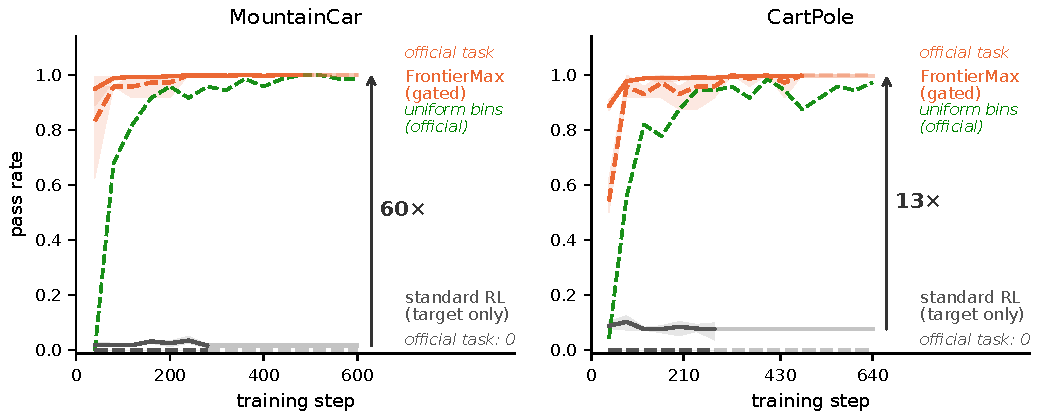
\includegraphics[width=\linewidth]{figures/fig6_gym}
\caption{\textbf{Gym control under binary task-success reward, trained
to plateau (3 seeds).} Solid: mean pass rate across curriculum bins;
dashed: the \emph{official} task (MountainCar flag / CartPole
survive-400). The target-only arm (gray) is a provable zero-update
freeze under sparse verifier-style reward; a uniform-over-bins control
(green) also cracks the task, $3\times$ slower and off-ceiling; the
gated FrontierMax stack converges to $1.000{\pm}0.000$.}
\label{fig:gym}
\end{figure}

\paragraph{6.6 gym control (full).} MountainCar flag: measured
random-policy success $< 3{\times}10^{-6}$ over $10^6$ episodes;
survive-400 ${\approx}10^{-13}$ by tail fit. Dense-reward controls
(prediction registered before the run): CartPole's native $+1$/step
reward lets vanilla REINFORCE on the same tile policy solve survive-400
($0.96{\pm}0.03$, 3 seeds); MountainCar's native $-1$/step reward
(constant until first success) stays at $0.000$ in all seeds --- the
categorical zero tracks reward sparsity, not the environment.
Attribution at a common 280-step horizon (hard-task AUC): MC $.750 \to$
+recycling $.895 \to$ +teacher $.956$; CartPole $.708 \to .792 \to
.893$; paired teacher increment positive 3/3 seeds on both;
creation-without-allocation plateaus at $0.958$ on CartPole in every
seed while adding the teacher restores $1.000$; teacher speed effect
$3.0\times$ to hard-task $0.9$ ($2.1\times$ to $0.99$ on CartPole).
The per-bin ablation replicates the 10-seed transition-matched study
(flag $0.848{\pm}0.058$) before strengthening it to full convergence.

\paragraph{6.6a Acrobot fixed-pool score test (fresh V2).}
A later source-locked CPU tournament uses official
\texttt{Acrobot-v1}, eight nested binary thresholds, one task-blind
H64 actor, practical MaxRL with $N{=}16$, no hindsight, and two
million paid transitions. Twenty fresh paired seeds compare uniform,
the common-scaffold $p(1-p){=}u_2$ score, and $u_{16}$. The registered
primary $u_{16}-p(1-p)$ target-uniform transition-AUC difference is
$+.04803$ (paired bootstrap 95\% CI $[+.02094,+.07385]$, exact
two-sided sign-flip $p=.003361$), clearing the predeclared $+.01$
point-estimate filter. Holm-controlled secondaries are $-.00616$ for
$p(1-p)-$uniform (adjusted $p=.50784$, not supported) and $+.04187$
for $u_{16}-$uniform (adjusted $p=.001617$, supported). This is a
score-shape result on a common sampler scaffold, not a full ProCuRL,
SFL, PLR, PAIRED, or ACCEL comparison. The exact test assumes sign
exchangeability; no miss is interpreted as equivalence.

\paragraph{6.6b Paid-probe ProCuRL confirmatory comparison.}
A separate source/runtime-locked family keeps the same eight thresholds, H64
actor, practical MaxRL estimator, $N=16$, and $3\times10^{-4}$ learning rate.
Its four arms are ordinary uniform; a paid-probe uniform sham; source-faithful
ProCuRL environment selection
$\operatorname{softmax}\{20\hat p(1-\hat p)\}$; and continuous-range-matched
$u_{16}$ selection. Probed arms estimate every task with 20 episodes initially
and at each crossed 5,120-student-transition boundary, charging every probe
transition to the nominal two-million paid budget. This 80-pair family and
five-secondary Holm plan are separate from the V2 score test above.

Across seeds 21000--21079, the internally frozen fixed-paid-AUC contrast
$u_{16}-$ProCuRL is $+.004894$ (paired SD $.022139$, $t_{79}=1.9773$,
$p=.05149$; 20,000-resample CI $[+.000110,+.009727]$; one-million
sign-flip $p=.05161$). It misses both the $.02$ SESOI and $.05$ paired-$t$
criterion. Holm-family contrasts are ProCuRL--sham $-.001704$ (adjusted
$p=.4568$), $u_{16}$--sham $+.003190$ ($.4547$), ProCuRL--ordinary
$-.313774$ ($3.47\times10^{-66}$), $u_{16}$--ordinary $-.308880$
($9.48\times10^{-67}$), and sham--ordinary $-.312070$
($4.06\times10^{-68}$). Fixed-paid arm means are $.33771$ (ProCuRL),
$.33942$ (sham), $.65149$ (ordinary), and $.34261$ ($u_{16}$).

The probed arms average 28.0--28.1 sweeps and only 140.5--141.1k student
transitions versus 2.003M for ordinary uniform; 93.19--93.21\% of their paid
transitions are probes. They receive 15.4--19.8 optimizer updates versus 259.1
for ordinary uniform. All 320 confirmation and 12 outcome-blind development
runs reconcile exactly, all 11 development gates pass, and the registered
common-random-number invariants replay. The result diagnoses probe-cost
domination for this learner and cadence; it does not establish full-PPO or
general ProCuRL inferiority.

The external confirmatory raw is 1,374,886,097 bytes. Its SHA-256 boundary is:
\begin{quote}\scriptsize
raw: \texttt{b1f8756c249effab8c77101c8bca73ddf708a5e143c18fe8742fd5712fdd7c12}\\
lock: \texttt{b7c7f76f6aaffa1fe65557717bfe545f2ec850495d370cd97fe72a8871fc8d0f}\\
analysis: \texttt{2010e30b5b15a212e2d6bdfaacd43d2434e5f468a96be613cf59744b9bc2fb38}
\end{quote}
The source bundle carries a 320-record external-raw receipt manifest: compact
verification checks the small-artifact bindings, while full verification
requires the raw and replays locked validation. The local lock is not an
immutable public pre-execution registration.


\begin{figure}[tb]
\centering
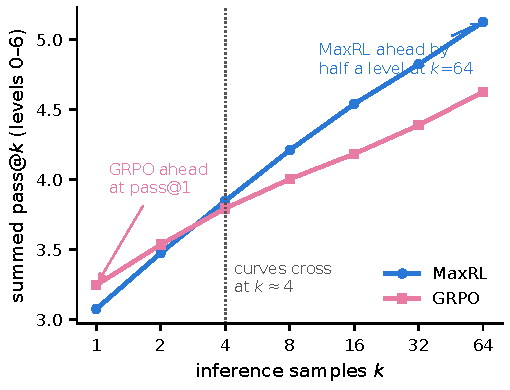
\includegraphics[width=0.55\linewidth]{figures/fig9_ksweep}
\caption{\textbf{Summed maze coverage vs.\ inference samples $k$
(final uniform-arm checkpoints).} GRPO leads at $\passat{1}$; the
curves cross at $k{\approx}4$; MaxRL leads by half a level at
$k{=}64$ --- choose the estimator by how many samples you will draw at
inference.}
\label{fig:ksweep}
\end{figure}

\paragraph{6.7 posterior diagnostics and harness caveats (full).}
The final steering-controlled cell passed the minimum dead-sampled
criterion ($.413<.50$) but missed the run-mean criterion
($.601480\not<.60$) by $.00148$; its endpoints are therefore
inconclusive by the pre-registered rule and are not interpreted.
The $\passat{k}$ sweep's absolute level sits ${\sim}3\times$ below the
trainer's val metric (unreconciled harness discrepancy; only the
within-sweep contrast is quoted). Posterior detail: two independent
teacher runs' posteriors agree with each other (cross-run Spearman
${\approx}.45$ on co-visited prompts, $n{\approx}900$; $\approx.67$
self-consistency with a shared latent) vs.\ $.10$--$.22$ against
external 7B-model annotations, from ${\sim}1.25$ visits per prompt.
Across external-difficulty quintiles spanning solve rates $.33 \to
.98$, mean $\hat p$ moves only $.076 \to .103$ --- the compressed
landscape that starves allocation. A response-length read we
advanced after five runs (three GRPO runs compressed harder than both
MaxRL runs) did \emph{not} survive the sixth: the within-seed control
run finished longer than every earlier run (252 vs.\ 208--236 tokens
from a common ${\sim}365$-token warmstart), so output length does not
separate the estimators at this scale and we withdraw it as a
sharpening signature. Prompt-uniqueness figures for the replacement confound:
${\sim}34\%$ unique prompts seen by teacher arms vs.\ ${\sim}43\%$
uniform.

\paragraph{Relabeling in a PPO-family loop: the wiring contract.}
For adopters (the details a config cannot express). \emph{Placement}:
relabeling runs after reward computation and \textbf{before}
\texttt{compute\_log\_prob} --- old log-probs must be computed under
the \emph{rewritten} conditioning, making the relabeled group an
on-policy ML term with the estimator's own weights, not a
policy-gradient ratio against stale context (our gridworld ablation
priced the stale-context mistake at $-0.06$ AUC, worse than no
hindsight). \emph{Rewrite}: the prompt's goal slot and the response's
goal mentions are both rewritten (token IDs, attention mask, and
position IDs rebuilt; 2-D RoPE only --- 3-D mrope is refused loudly);
the answer artifact is untouched by construction. \emph{Group
semantics}: each parseable failure relabels to its own achieved goal
and keeps its group id, so one group can mix relabeled tasks;
unparseable rollouts stay failures, preserving contrast ($K<N$). The
group contrast is then ``reached some verified goal'' vs.\ ``reached
none'' --- coarser than 1-of-$N$ of a single task, pre-registered as a
deviation, with the verl-normalized advantage verified equal to
$N\times$ the reference weights in direction; as
Remark~\ref{prop:hindsight} states, this per-row variant is a
weighted-SFT update, not a per-destination MaxRL gradient.
\emph{Hygiene}: the
curriculum posterior observes pre-relabel scores only; no KL-to-
reference is applied to relabeled groups in our runs
(\texttt{kl\_coef=0}). Reference implementation vendored in this
repository (\texttt{verl\_integration/vendored/hindsight.py},
${\sim}270$ lines, with execution-commit provenance and CPU
integration tests). We preserve that reported-run snapshot byte for
byte. For new runs, the release entry point
\texttt{verl\_integration/hindsight.py} inherits the snapshot but
replaces its broad response-number substitution with a conservative
goal-statement rewriter: signed values, decimals, arithmetic, unknown
contexts, and \texttt{<answer>} blocks remain untouched. Twenty-six
CPU regression/property tests cover these contracts.

\paragraph{Jugs suite (pool-conditionality; \S\ref{sec:limits}).} Tier grid t0--t4
(2--5 jugs, disjoint min-moves bands, 200 unique tasks/tier);
feasibility landscape (SmolLM2-360M two-shot, $N{=}16$): t0
$.058/.475$ (mean@16/bootstrap best@16 proxy), t1 $.006/.100$, t2--t4 $0/0$ with
relabel-yield-on-failure $.62$--$.73$ on every tier. All nine
pre-registered B-arm cells (no-recycling / ungated / gated $\times$ 3
seeds) converged to the same deterministic fixed point: t0
mean@16$\,=\,$bootstrap best@16 proxy$\,=0.450$ exactly (the 2-move
template stratum), t1 bootstrap best@16 proxy $0.15 \to 0$, actor entropy
$1.36 \to 0.02$--$0.21$.
Ungated recycling ran 169 relabels/step at yield $.88$ and ended with
the lowest entropy ($0.02$--$0.03$); the value-keyed gate rejected
$99.8\%$ of relabels (the granularity bug described in \S\ref{sec:limits}, since
fixed and regression-tested). Fig.~\ref{fig:jugs} shows all nine
trajectories: the collapse is the pool's property, not any
intervention's. Postmortem and per-cell artifacts in the
repository.

\begin{figure}[tb]
\centering
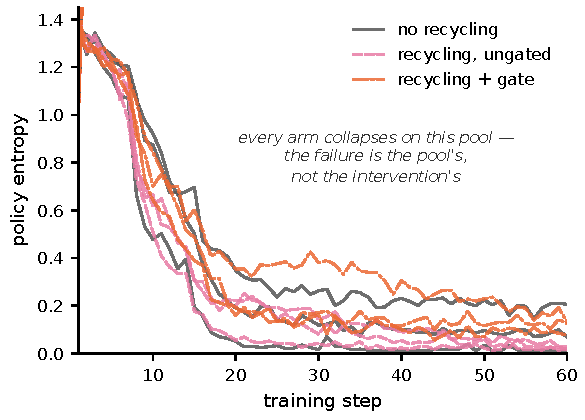
\includegraphics[width=0.55\linewidth]{figures/fig10_jugs_entropy}
\caption{\textbf{Jugs pool-conditionality: every arm collapses
(3 arms $\times$ 3 seeds).} On a pool whose learnable band is a
single stratum of 1--2-move template solutions, plain MaxRL's policy
entropy collapses ($1.36 \to 0.01$--$0.21$) with no recycling
involved; ungated recycling ends lowest, and the gate merely delays
the fall. Rollout-set diversity at initialization is the design gate
this suite motivates (\S\ref{sec:limits}).}
\label{fig:jugs}
\end{figure}

\paragraph{6.9 secondary reads (full).} Pool construction and
baseline calibration: the pre-SFT base model's relabel yield is
$0.000$ ($n{=}384$) --- the syntactic prerequisite; post-SFT the
model is a near-independent guesser whose bootstrap best@16 proxy sits at a
tier-invariant ${\sim}75\%$ of the independence bound
$1-(1-\mathrm{mean@16})^{16}$ (ratios $.744/.783/.755$ across tiers), the
baseline the headroom gate measures against. Training-side damage: ungated
recycling ends with more unsolvable-at-16 frontier training prompts
than baseline in every seed (paired $+.083/+.063/+.034$). Entropy at 3
seeds: the gate's retention replicates ($+.072$ paired over baseline,
all seeds positive, ${\sim}1.6\times$); ungated recycling's endpoint
entropy is seed-unstable (spread $\pm.062$, $4$--$9\times$ the other
arms'), consistent with its noisy frontier-coverage endpoints.
Designed-strength sweep (P-R1) per-seed tier-1 endpoints
(mean@16/bootstrap best@16 proxy, rejection fraction): $.212/.513$ ($.934$),
$.322/.573$ ($.934$), $.264/.488$ ($.944$) --- the registered windows
were mean-kept $\in [0,.60]$ of B2's gain and coverage
$\in [.541,.571]$; observed mean-kept $-0.25$, coverage proxy $.525$.
Artifacts \texttt{armA\_b3fix\_s\{1,2,3\}.json} with protocol and
verdict documents in \texttt{countdown\_reviewer\_arms/}.

\section{Claims and evidence}\label{app:claims}

Every load-bearing claim, its strongest evidence, and its externally recorded
registration status. For maze wave 2 and the Countdown controls, the release
contains protocol and verdict documents but not the locking commit objects;
their timing cannot be independently audited from this checkout. Artifacts
named per row live in the repository with the run registry
(\texttt{run\_registry.json}).

\begin{table}[h]
\centering\footnotesize
\setlength{\tabcolsep}{3.5pt}
\caption{Claim inventory. $\uparrow$ = met the stored directional rule;
$\downarrow$ = refuted, committed branch executed; $\circ$ =
descriptive/exploratory; ``inc.'' = inconclusive because a
pre-registered treatment-delivery gate failed.}
\label{tab:claims}
\begin{tabular}{@{}p{0.32\linewidth}p{0.38\linewidth}cl@{}}
\toprule
claim & strongest evidence & status & where \\
\midrule
mass identity $A_N = 2u_N$; factorization
$\mathbb{E}[\hat g|x] = u_N(\mu_+{-}\mu_-)$ & proof + MC
(\texttt{verify\_guidance\_math.json}); enumeration test in CI &
proved & Prop.~1 \\
drop-$K{=}0$ estimator unbiased for $T{=}N{-}1$ & three-line
derivation + SymPy check & proved & Lem.~1 \\
allocation saturates: oracle ties full stack & no-floor
$\gamma$-matched oracle $.8885 \approx .8895$, 5 seeds & $\circ$ &
\S 6.1 \\
rollout awareness matters beyond $N{=}2$ & fixed-completion sweep:
$u_2=p(1-p)$ exactly; $u_N>p(1-p)$ in 8/8 paired seeds for every
$N\in\{4,8,16,32\}$ & $\circ$ post-guidance & \S 6.1 \\
paid-probe $u_{16}$ superiority over ProCuRL selection & separate 80-pair
family: $\Delta=.004894$, $p=.05149$, below SESOI $.02$; all probed arms
about $.31$ AUC below ordinary uniform & $\downarrow$ unsupported & \S 6.6b \\
creation is the only live channel at $p{\approx}0$ &
uniform+recycling $.931 \approx$ teacher+recycling $.928$ vs.\
$0.000$ all pure samplers, 5 seeds & $\circ$ & \S 6.2 \\
zero-exception coverage divergence (9-run cohort) & failed balanced
factorial at registered endpoint (3/6, 4/6 vs.\ $\ge$5/6 both) &
$\downarrow$ retracted & \S 6.3b \\
time-integrated coverage ordering (MaxRL $>$ GRPO) & wave-2
registered primary on fresh blocks: 6/6 per sampler, $p{=}.031$
each; block mean $+.01950$, 95\% interval
$[+.01148,+.02752]$; 12/12 block averages positive descriptively
across waves & $\uparrow$ & \S 6.3b \\
easy-band localization of GRPO's loss & P-F3 met its registered
pair-level bar (10/12), but block-level 4 positive/1 tie/1 negative
and interval includes zero & $\circ$ suggestive & \S 6.4 \\
variance normalization is the tail mechanism & exact rung: no-SD
GRPO collapses onto RLOO ($.148$ vs.\ $.161$); neural rung: P-G0c
\emph{failed} (loses easy band 6/6) & split & \S 6.3b--6.4 \\
GRPO's own-mass teacher doesn't rescue it & P-G0a confirmed 5/6,
both rungs & $\uparrow$ & \S 6.3b \\
exact-rung ordering survives lr recalibration & P-LR1 falsified as
registered: $2$--$4\times$ lr closes raw $\Delta$cov but premium
collapses ($.007$--$.013$ vs.\ $.050$) --- restated at-matched-lr &
$\downarrow$ & \S 6.3b \\
recycling-package concentration (mean up, bootstrap proxy down) &
three-seed aggregates; standard pass@$k$ unavailable; exploratory seed-1
proxy curve & $\circ$ metric-limited & \S 6.8 \\
higher-dose live-group alternative at LLM scale & replay (2 epochs) improves
both logged metrics but does not isolate dose or direction & $\circ$ confounded
& \S 6.8 \\
under-gated setting is a candidate operating point & frontier-tier
coverage to baseline at ${\sim}60\%$ mean kept, but faulty decay,
3 seeds & $\circ$ & \S 6.9 \\
gate strength is a monotone dial & designed-strength sweep P-R1:
mean-kept $-0.25 \notin [0,.60]$, coverage proxy $.525 < .541$, 3 seeds &
$\downarrow$ & \S 6.9 \\
estimated-$p$ gate is affordable & P-PB1 confirmed: one probe
rollout/step recovers 98\% of the oracle-vs-frequency gap at matched
total rollouts (10/10) & $\uparrow$ & \S 6.9 \\
LLM teacher$\times$estimator interaction (GSM8K) & controlled cell
missed run-mean treatment gate by $.00148$; endpoint uninterpretable &
inc. & \S 6.7 \\
pool-conditionality: Jugs defeats every arm & pre-registered
all-null with entropy-collapse mechanism & $\uparrow$ &
\S\ref{sec:limits} \\
\bottomrule
\end{tabular}
\end{table}

\section{Hyperparameters and compute}\label{app:hparams}

Total compute for every experiment in this paper: ${\sim}230$
A10G-hours on a single GPU plus CPU-days for the exact-gradient suites.
Step-time telemetry (artifact \texttt{generation\_timing.json}, 1{,}188
mixed GSM8K/Countdown steps): step-weighted mean generation fraction
31\% overall; the eight generation-dominated sessions ($>$80\% session
mean, 282 steps) average 83\% --- a selected-subset description, not
an estimate of typical cost. Table~\ref{tab:suites} gives the
per-suite configuration and Table~\ref{tab:knobs} the knob inventory
with provenance.

\begin{table}[h]
\centering\small
\caption{Per-suite configuration. Teacher knobs (decay, floor, $\gamma$)
are shared across suites with the defaults below; what varies per suite
is scale, not schedule.}
\label{tab:suites}
\begin{tabular}{@{}lllll@{}}
\toprule
 & chains (\S6.1--6.2) & maze (\S6.3--6.4) & GSM8K (\S6.7) & Countdown (\S6.8--6.9) \\
\midrule
policy & exact tabular & 1.26M transformer & SmolLM2-360M & SmolLM2-360M (SFT) \\
rollouts $N$ & 16 & 32 & 16 & 16 \\
groups/step & 1 & 8 & 64 & 64 \\
optimizer, lr & SGD, 0.5 & AdamW, $10^{-4}$ & AdamW, $10^{-5}$ & AdamW, $10^{-5}$ \\
budget & 3{,}200 groups & 2{,}400 s / 250 steps$^{\dagger}$ & 50 steps & 60 steps \\
seeds (headline) & 5--10 & 3 / 6 blocks$^{\dagger}$ & 1--2/cell & 3/arm \\
compute/run & CPU-min & 0.7 A10G-h & ${\sim}20$ A10G-h & ${\sim}6$ A10G-h \\
\bottomrule
\end{tabular}

\smallskip
{\footnotesize $^{\dagger}$cohort runs (\S 6.3a) used 2{,}400 s
wall-clock; the balanced factorial and its confirmation wave use 250
fixed steps (matched generation and optimization budget) over six seed
blocks --- the two protocols are never mixed within a comparison.}
\end{table}

\begin{table}[h]
\centering\scriptsize
\setlength{\tabcolsep}{2pt}
\caption{Teacher and recycler knobs: value, provenance, and measured
sensitivity.}
\label{tab:knobs}
\begin{tabular}{@{}p{0.22\linewidth}p{0.10\linewidth}p{0.22\linewidth}p{0.38\linewidth}@{}}
\toprule
knob & default & derived or tuned & sensitivity \\
\midrule
peak location/$N$-scaling & --- & \textbf{derived} (Prop.~1) & the theory claim \\
posterior decay & 0.7 & tuned (V2b) & closes ${\sim}19\%$ of oracle gap \\
uniform floor & 0.1 & tuned & 0.15 on maze; robust 0.05--0.2 \\
$\gamma$ (concentration) & 1 & tuned (V6) & 4 on chains; no transfer to maze \\
\texttt{gate\_max\_p} & 0.5 & tuned ($p{=}1$ zero vacuous) &
under-gated point only; corrected strong arm failed (\S6.9) \\
relabel dose cap & 12 groups/step & tuned & sets \emph{where} coverage is spent (\S6.4) \\
\bottomrule
\end{tabular}
\end{table}

\section*{Reproducibility}
One command verifies the artifact end to end:
\texttt{bash reproduce.sh} runs the proposition and integration
tests, validates the generated run registry and overlap/rewrite audit
tools, re-derives the figure endpoints that have retained per-seed artifacts
(failing on mismatch), checks every manifest checksum, regenerates
every figure from its frozen inputs, and spot-checks each quoted
stored protocol/verdict numbers against the corresponding artifacts
(\texttt{--build} additionally rebuilds both PDF wrappers).
Every proposition has an enumeration/Monte-Carlo verification script
(\texttt{test\_mass\_formulas.py} in \texttt{curriculum\_maxrl/}
checks the MaxRL, RLOO, and both GRPO-SD mass formulas against exact
enumeration and the deployed code). Figure sources, checksums, and
commands are listed in the frozen
\texttt{paper/results/manifest.json}; most result values live in
versioned JSON tables. Known exceptions are stated here rather than
hidden: Fig.~\ref{fig:passk} reads a checksummed structured input containing
the single-seed logger transcription and session provenance, but remains
exploratory until replaced by structured three-seed outcomes; the maze cohort
of Fig.~\ref{fig:bands} is frozen in an explicit
run manifest --- adding a run file cannot silently change the figure,
and missing inputs are a hard error. The Jugs preregistration, raw
cells, verdicts, and postmortem are vendored in
\texttt{jugs\_llm/results/} with preregistration- and execution-commit
provenance. The LLM-scale relabeling implementation is vendored
verbatim with execution-commit provenance
(\texttt{verl\_integration/vendored/}), so the loop the Countdown and
Jugs suites executed is inspectable in this repository. Known gaps,
stated rather than papered over: the IsaacLab
pilot is reported from an independent team's summary (raw logs live
with that team); per-step timing fractions come from verl's in-run
telemetry (\texttt{generation\_timing.json}); the fig2/fig3 endpoint
tables were transcribed from run analyses, and all of fig2's
quantitative panels now carry checked-in derivation scripts that
regenerate them from per-seed artifacts and fail on mismatch
(\texttt{verify\_fig2a\_from\_artifacts.py} covers panels a--b,
\texttt{verify\_fig2c\_from\_logs.py} panel c against raw maze seed
logs) --- only the GSM8K panel (d) and fig3 remain transcribed, with
per-panel provenance in the data files; and
the GSM8K pass@$k$ harness sits
${\sim}3\times$ below the trainer's val metric (unreconciled; only
within-sweep contrasts are quoted). The schema-v2 one-row-per-run
registry (\texttt{curriculum\_maxrl/run\_registry.json}) contains 562
run records supported by local artifacts, receipts, or summaries: 94 maze, 20
Countdown, 7 GSM8K, and 441 Acrobot,
including all balanced-factorial cells, Countdown replay seed 3, and
the completed GSM8K steering-controlled cell. It distinguishes 33 individual
vendored run-level files, 121 Acrobot run records embedded with per-run
diagnostics in vendored aggregates, 320 paid-probe confirmation rows bound by
per-run receipts to the 1.375 GB external raw, and 88
summary/external-backed rows. The receipt manifest binds raw SHA-256
\texttt{b1f8756c249effab8c77101c8bca73dd\allowbreak{}f708a5e143c18fe8742fd5712fdd7c12};
compact verification checks its small-artifact boundary and full verification
requires the raw and replays all 320 ledgers. The Acrobot total comprises 40
historical V3, 9 V2 development, 60 V2 confirmation, 12 paid-probe
development, and 320 paid-probe confirmation runs;
missing raw logs are explicit rather than
silently claimed. The maze main-effect subset and
its 5v4 composition are tabulated in
\texttt{permutation\_reanalysis.json}, committed alongside. Data
hygiene is separated by stage. The RL train/eval pools carry zero
overlap and zero intra-split duplicate tasks. A stored summary reports that 27
of 128 Countdown tier-0 evaluation tasks overlap the SFT warm start and zero
measured overlap for tiers 1--2; the missing source manifests prevent
independent recomputation. The schema-v2 integrity record marks the
full-128 tier-0 absolute metrics contaminated and exposes the 101-task
clean subset. A numeric clean-subset reanalysis remains blocked because
this checkout lacks the frozen SFT/evaluation manifests and the 16
per-task verifier outcomes (or compatible checkpoints) for each arm
and seed; aggregate tier endpoints cannot recover that subset. The
framework is a dependency-light package (\texttt{frontier\_rl},
numpy-only core) with adapters for LLM pools (verl), gym control,
IsaacLab parallel sim, and flow-policy VLAs.
